
%%%%%%%%%%%%%%%%%%%%%%% file typeinst.tex %%%%%%%%%%%%%%%%%%%%%%%%%
%
% This is the LaTeX source for the instructions to authors using
% the LaTeX document class 'llncs.cls' for contributions to
% the Lecture Notes in Computer Sciences series.
% http://www.springer.com/lncs       Springer Heidelberg 2006/05/04
%
% It may be used as a template for your own input - copy it
% to a new file with a new name and use it as the basis
% for your article.
%
% NB: the document class 'llncs' has its own and detailed documentation, see
% ftp://ftp.springer.de/data/pubftp/pub/tex/latex/llncs/latex2e/llncsdoc.pdf
%
%%%%%%%%%%%%%%%%%%%%%%%%%%%%%%%%%%%%%%%%%%%%%%%%%%%%%%%%%%%%%%%%%%%


\documentclass[runningheads]{llncs}

\usepackage{amssymb}
\setcounter{tocdepth}{3}
\usepackage{graphicx}
\usepackage{hyperref}
\usepackage{url}
\usepackage[english]{babel}
\usepackage{graphicx}
\urldef{\mailsa}\path|{aysengupta, xianlin, ksanjeev, sravichandra}@cs.stonybrook.edu|
\newcommand{\keywords}[1]{\par\addvspace\baselineskip
\noindent\keywordname\enspace\ignorespaces#1}
\newcommand{\swallow}[1]{ }

\begin{document}

\mainmatter  % start of an individual contribution

% first the title is needed
\title{Final Report: Team 8\\
Predicting Prices of Oil and Gold}

% a short form should be given in case it is too long for the running head
\titlerunning{Predicting the Prices of Oil and Gold}

% the name(s) of the author(s) follow(s) next
%
% NB: Chinese authors should write their first names(s) in front of
% their surnames. This ensures that the names appear correctly in
% the running heads and the author index.
%
\author{Ayush Sengupta \and Benjamin Lin \and Komal Sanjeev \and Sreevathsan Ravichandran}
%
\authorrunning{Ayush Sengupta \and Benjamin Lin \and Komal Sanjeev \and Sreevathsan Ravichandran}
% (feature abused for this document to repeat the title also on left hand pages)

% the affiliations are given next; don't give your e-mail address
% unless you accept that it will be published
\institute{Department of Computer Science, Stony Brook University,\\
Stony Brook, NY 11794-4400\\
\mailsa\\
\url{http://www.cs.stonybrook.edu/~skiena/591/projects}}

%
% NB: a more complex sample for affiliations and the mapping to the
% corresponding authors can be found in the file "llncs.dem"
% (search for the string "\mainmatter" where a contribution starts).
% "llncs.dem" accompanies the document class "llncs.cls".
%

\toctitle{Lecture Notes in Computer Science}
\tocauthor{Authors' Instructions}
\maketitle

\swallow{   % DO NOT BOTHER WITH THIS
\begin{abstract}
The abstract should summarize the contents of the paper and should
contain at least 70 and at most 150 words. It should be written using the
\emph{abstract} environment.
\keywords{We would like to encourage you to list your keywords within
the abstract section}
\end{abstract}
}


\section{Challenge} 

Our challenge is to predict the prices of Oil and Gold on January 1st 2015 as of December 1st in 2014 (a month in advance). 

\subsection{Oil}

Oil is a non-renewable resource which occurs in the earth. It is extracted and sent to refineries where different petroleum products such as gasoline, petrol, heating oil, etc are separated. Almost two-thirds of our energy demands are met by oil. Oil is the most heavily and actively traded commodity, which accounts to almost 10\% of the world's trade.\\

\noindent The price of oil is determined by supply and demand. An increase in demand results in an increase in the price of oil. The supply and demand themselves are determined by various factors such as economy, weather and geopolitics. \\

\noindent Being an extensively traded commodity, coupled with several factors which affect its price, the oil price is very volatile. Some of the factors might even be interdependent, which makes it very difficult to estimate the extent to which an individual factor could affect the price. Moreover, the relationship between certain factors and the oil prices could also change over time. These factors make the prediction of oil prices a very complex and challenging problem.

\subsection{Gold}
Gold is viewed as a symbol of wealth since the ancient times of the human history. It is widely used as jewelry and in some precision gages. \\

\noindent For the long period of time, the gold price is fixed; until 1968, with the breakdown of Bretton Woods Currency Arrangement, the gold price started to be market determined. People also invest in gold, especially when the melt-down of US dollars, becasue gold plays a signifanct role as a stabilizing influence for investment portfolio. \\

\noindent The gold price faces similar challenges as the oil price. It is dynamic and highly volatile. Multiple factors affect the gold price. The extent of correlation and the level of importance of each factor are not clearly known. Also similar to the difficulties we face in oil price prediction, some of these factors are interdependent, so we need to estimate the level of inter-correlation between them. 

\section{History/Background}
\subsection{Factors Affecting the Price of Oil}
Crude oil prices are determined by the balance between supply and demand. An increase (or decrease) in demand causes the price of oil to rise (or fall). Consequently, a cutback in the production of oil results in an increase in oil prices. There are several factors which disturb the supply-demand balance, thus resulting in oil price fluctuations. 

\subsubsection{Organization of the Petroleum Exporting Countries (OPEC) Supply}
OPEC is an organization of 12 oil exporting nations, namely Algeria, Angola, Ecuador, Iran, Iraq, Kuwait, Libya, Nigeria, Qatar, Saudi Arabia, United Arab Emirates, and Venezuela. It aims at coordinating and unifying petroleum prices of its member countries \cite{opec}.Oil supply from the OPEC member countries represents about 40\% of the world’s crude oil, and their actions can affect the prices of oil to a significant extent. For example, limiting the oil production from OPEC’s major oil producers such as Saudi Arabia can influence crude oil supply and affect the prices \cite{eiafactors}.\\\\ 
\noindent Oil prices not only depend on the current demand and supply, but also on the projected future supply and demand. OPEC adjusts the oil productions of its member countries based on current and future demand.

\subsubsection{Non-OPEC Supply}
The non-OPEC countries produce about 60\% of the world's crude oil. A lack of supply from the non-OPEC countries creates additional pressure on the OPEC countries which can also contribute to a rise in oil prices \cite{eiafactors}.

\subsubsection{Stock Price}
As economic conditions improve, there is an increase in demand for several commodities including oil, which results in an increase in oil prices. The Standard and Poor's 500 (S\&P 500) index is a common benchmark for the stock market of USA. It is a weighted index of the market capitalization of 500 companies. It is the most commonly used indicator of the US economy.

\subsubsection{Market Transactions - Spot price and Futures}
The current price at which a commodity can be traded at a specific place and time is called the spot price. Crude oil can be purchased on the spot at the current market price. \\\\
Crude oil can also be traded in the futures market. A futures market is when a commodity is traded in futures contracts, i.e., a contract between a buyer and seller where the buyer agrees to buy a certain quantity of a commodity for a fixed price at a time in the future. \\\\
The uncertainity of futures contract prices tend to affect the spot oil prices.

\subsubsection{Seasonal Effects}
Certain crude oil products such as heating oil and gasoline tend to have a seasonal variance. For example, there is an increase in demand for oil in the fourth quarter due to the cold weather, and a subsequent reduction in demand during late winter as the weather gets warmer. Gasoline prices also tend to rise in the summer due to an increased consumption. 

\subsubsection{US Dollar Exchange Rate (USDX)}
Oil is traded in Dollars, and thus, any change in the Dollar exchange rate relative to other currencies can cause oil prices to shift. Several studies support the negative correlation between the  dollar exchange rate and the price of oil. There are several arguments to support this statement. One reason could be that the depreciation in the dollar exchange rate causes the oil to be cheaper in countries outside the US, thus leading to an increase in demand, which in turn causes oil prices to rise. However, it has been observed that the relationship between oil prices and the dollar exchange rate has not been stable over the years \cite{eiafactors} \cite{oildollar}.

\subsection{Factors Affecting the Price of Gold}
Gold is a precious metal which was used as a currency in several major civilizations in the past centuries. In the Unites States of America, gold had been at a fixed price of about \$20 per ounce, since the early 19th century. In 1934, President Franklin Roosevelt raised gold price from \$20.67 per ounce to \$35. In 1968, with the breakdown of Bretton Woods Currency Arrangements, the gold price became market determined. From \autoref{fig:Gold_since1970.png} below, we observe that the two peaks of the gold price coincide with two significant economic recessions in our history - one in 1980, and the other 2008.\\

\begin{figure}
\centering
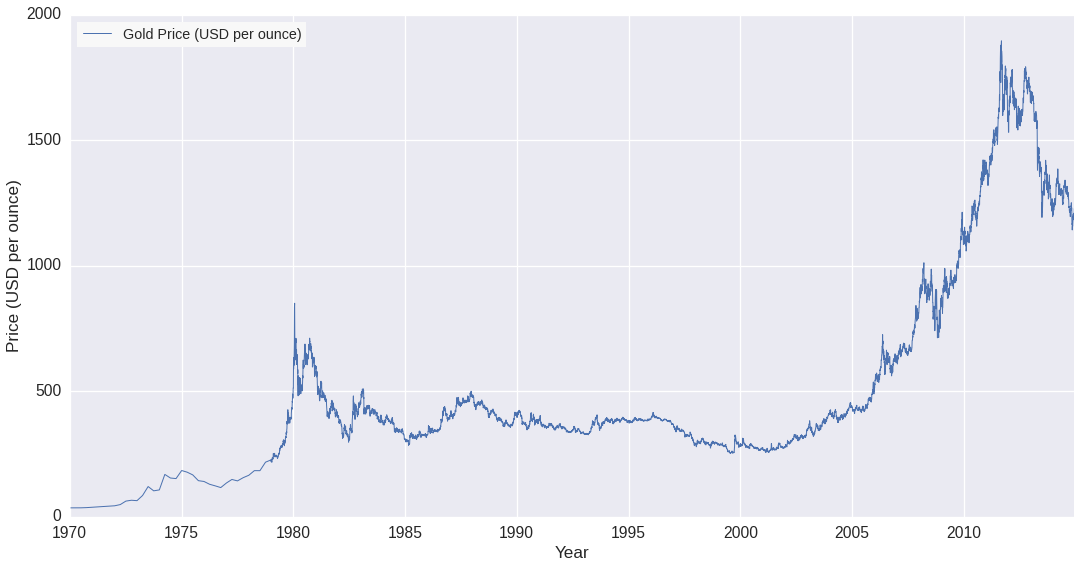
\includegraphics[width=\textwidth]{Gold_since1970.png}
\caption{Gold price in dollars per ounce from Jan 1, 1970 to Dec 9, 2014}
\label{fig:Gold_since1970.png}
\end{figure}

\noindent Based on our paper review, we found the following 9 factors would affect the gold price: Crude Oil Price, Commodity Research Bureau future index (CRB), EURO/USD Foreign Exchange Rate (EURO/USD), Inflation rate (INF), Money Supply (M1), and US Dollar index (USDX) \cite{gold-shafiee}\cite{gold-zhang}\cite{gold-Ismail}. In the model development process, we selected some of them to be included in our models.

\subsubsection{Inflation}
In history, during inflation, people tended to keep precious commodities such as gold instead of paper money to ensure their assets were not reduced too much. Therefore, the higher the inflation is, the higher the gold price is in general.

\subsubsection{Stock Price}
Similar to the oil price case, NYSE and S\&P 500 indexes are common benchmarks for the US economy.

\subsubsection{US Dollar Exchange Rate (USDX)} 
Similar to the oil price case, US dollar is the currency in trading gold. The raise of the USDX implies an increase of the US dollar purchasing power, which reduces the consumers' motivation of keeping gold, and possibly decreasing the gold price.

\subsubsection{Consumer Sentiment Index (CSI)} 
The Consumer Sentiment Index or Consumer Confidence Index, is an index measuring the consumers' confidence over the market \cite{csi-1}\cite{csi-2}. Similar to the effects of USDX over the gold price, a high CSI indicates consumers generally feel optimistic about the overall economy and their ability of obtaining and keeping their jobs, so they would be less likely to keep precious metals like gold.

\subsubsection{Crude Oil Price}
Crude oil prices have an approximate 85\% to 92\% correlation with gold prices. Rising oil prices may lead to an increase in the gold price, but the converse may not be true \cite{gold-shafiee}\cite{gold-zhang}.
The gold-oil relation suggests that the crude oil price could partly account for inflation. An increase in the oil price results in increased prices of gasoline. Gasoline being more expensive results in an increase in the cost to transport goods, thus causing a possible hike in prices of goods. The final result is an increased price level – in other words, inflation. Gold tends to appreciate with inflation. Therefore, elevated oil prices can eventually lead to higher gold prices \cite{gold-url1}. 

\begin{figure}
\centering
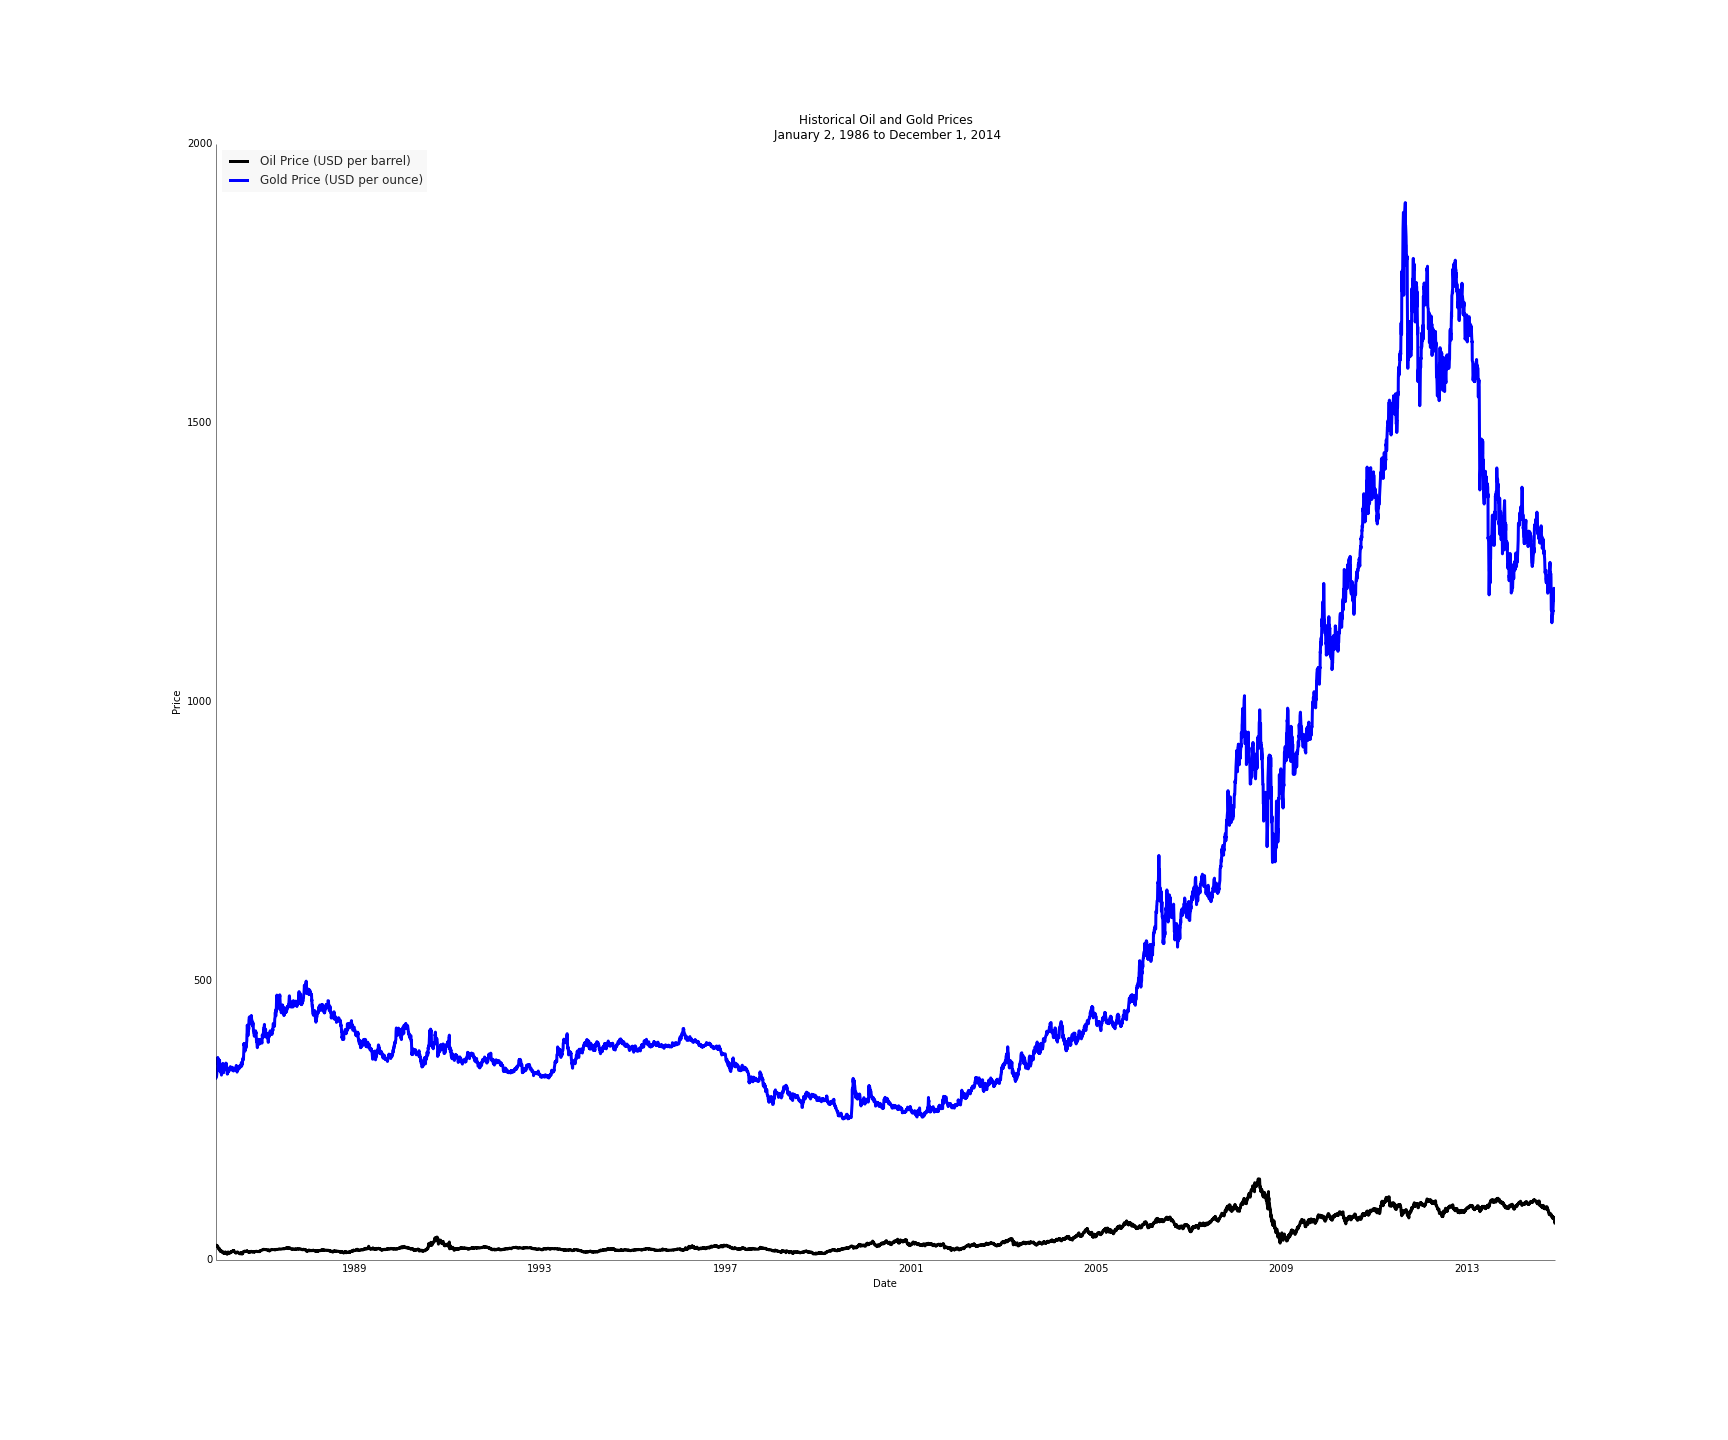
\includegraphics[width=\textwidth]{OilvsGold.png}
\caption{Historical Oil and Gold Prices (1986-2012) show a correlation, particularly before 2009}
\label{fig:OilvsGold.png}\begin{flushright}\end{flushright}
\end{figure}

\section{Literature Review}
There is a significant amount of papers aiming on undersanding and predicting oil and gold prices. Various studies have developed different prediction models based on different techniques and factors. Some studies try to make predictions based on historical oil and gold prices. Others focus on the economic aspects and try to explain the correlations between the prices of oil and gold with respect to a variety of economic factors. Therefore, we evaluate and summarize some widely used models into the following two categories: Standard Time Series Models and Structural Models Considering Economic Factors.

\subsection{Standard Time Series Models(Technical Models)}
Standard time series models attempt to predict the oil price using the current and historical oil prices. The same strategy applies to predicting the gold price as well. This type of models is useful in the following conditions:\\
\textbf{1.} The prices show autocorrelation and autoregressive behavior, i.e., there is a pattern or a significant correlation between current and the previous prices.\\
\textbf{2.} There are a large number of explanatory variables and it is difficult to understand them well because they interact with each other in a very complicated manner.\\
\textbf{3.} Forecasting the dependent variable may require predicting the explanatory variables. And prediction of the explanatory variable might in turn be a harder problem.\\
\textbf{4.} Not all explanatory factors and variables are known.\\ 

\noindent The most basic time series models that have been applied to model oil prices are the autoregressive models. In general, an autoregressive model \textbf{AR(p)} tries to model the current value of a time series based on the value of the last 'p' instances in the time series.\\

\noindent Thus, $ X_{t} = c + \sum\limits_{i=1}^p \varphi_{t-i}X_{t-i} + \epsilon_{t}$.\\\\

\noindent The co-efficients are regressed to predict the current price. Here the term $\epsilon_{t}$ is known as the \textit{white noise}. It is a random variable with zero mean, constant variance. Also, $corr(\epsilon_t,\epsilon_{t-1})$ is $0$ $\forall i>1$ and it is $1$ for $i=0$. In other words, $\epsilon_{t}$ is a random variable with no auto-correlation.\\

\noindent Similarly, Autoregressive–moving-average (ARMA) models take in to account the moving average factor. They try to predict the randomness based on the historical prices.  Hence \textbf{ARMA(p,q)} can be written as:\\

$ X_{t} = c + \sum\limits_{i=1}^p \varphi_{t-i}X_{t-i} + \epsilon_{t} + \sum\limits_{i=1}^q \theta_{t-i}X_{t-i}$.\\
\\

\noindent Further, it is known that oil price changes(volatility) follow GARCH/ARCH properties. Least square models generally assume that the expected value of all error terms, when squared, is constant. This assumption is termed as homoskedasticity. Data(time series) in which this conditions fail to hold, are heteroskedastic. ARCH and GARCH models treat heteroskedasticity as a variance which is then modelled autoregressively.\cite{engle}\\

\noindent In short, GARCH models split the error-terms $\varepsilon_t$ into a stochastic component $z_{t}$ and a time dependent variance $\sigma^2_{t}$. Thus, $ \varepsilon_t = z_{t} + \sigma_{t}$. The series $\sigma^2_{t}$ in \textbf{ARCH(q)} is modelled by:\\\\

$\sigma^2_{t} = \alpha_{0} + \sum\limits_{i=1}^q \alpha_{i}\varepsilon_{t-i}^2 $\\\\

\noindent Similarly \textbf{GARCH(p,q)} is modelled by:\\\\

$\sigma^2_{t} = \alpha_{0} + \sum\limits_{i=1}^q \alpha_{i}\varepsilon_{t-i}^2 + \sum\limits_{i=1}^p \beta_{i}\sigma_{t-i}^2 $\\\\

\noindent GARCH and ARCH models have consistently been used in the literature to predict oil prices with varying degrees of accuracy. 

\subsection{Structural Models Considering Economic Factors}

For the price of oil, structural models consider the oil price to be modelled as a function of certain explanatory variables such as oil consumption and production, OPEC behaviour, interest rates, exchange rates, and other commodity prices. The major drawback of using structural models to predict oil prices is that the models are extremely complex, and there is a strong inter correlation between factors themselves. Hence, there have not been many studies that focus on structual analysis to forecast oil prices.\\

\noindent According to Huntington(1994)\cite{huntington}, structural demand and supply models are generally not successful in predicting oil prices due to inaccurate forecasts of GDP and the oil supply from different countries. Another reason was not taking into account the market participation expectation of OPEC countries. \\

\noindent However, some interesting work has been done based solely on structural models. Most of these studies use models and results that instead of trying to predict the price, try to understand the nature of the oil market. Also, these models predict short-term oil prices, and it is unclear if they could be used for long term forecasting. One such interesting study by Pindyck(1999)\cite{pindyck} shows that long term oil prices are mean reverting around shifting trend lines. \\

\noindent In another direction Yang et al.(2002) \cite{yang} introduces a model to determine the factors affecting US oil prices. First, they highlight the unstable demand structure of the oil market. Then, they use a GARCH model (general autoregressive conditional heteroskedasticity) to investigate the volatility of oil prices. Using the co-efficients they generated, they estimate that the future oil price will be $0.987$ times the current oil price if the US GDP decreases by $5\%$. \\

\noindent Similarly, structural models considering a variety of economic factors also apply to the gold price prediction. According to Ismail et al.(2009)\cite{gold-Ismail}, they design models with the gold price as the only dependent variable, alongside different numbers of independent variables. Initially, they propose that the gold price is dependent on the following 8 factors: Commodity Research Bureau future index (CRB), USD/Euro Foreign Exchange Rate (EUROUSD); Inflation rate (INF); Money Supply (M1); New York Stock Exchange (NYSE); Standard and Poor 500 (SPX); Treasury Bill (T-BILL) and US Dollar index (USDX). Therefore, their first-order regression model, which they call it naive model, is like: \\

$\hat{Y}=-560.618+0.712X_1+161.740X_2-7.836X_3 +0.424X_4-0.010X_5+0.010X_6+3.198X_7+0.580X_8$ \\\\
where $\hat{Y}$ is the predicted gold price; $X_1$ is CRB; $X_2$ is EUROUSD; $X_3$ is INF; $X_4$ is M1; $X_5$ is NYSE; $X_6$ is SPX; $X_7$ is T-Bill; $X_8$ is USDX.\\

\noindent Then they show that using stepwise regression, the number of independent variables can be reduced from 8 to 4. Their enhanced model is  \\

$\hat{Y}=-301.509+0.676X_1+114.651X_2-5.563X_3+0.309X_4$ \\\\
where $\hat{Y}$ is the predicted gold price, $X_1$ is CRB; $X_2$ is EUROUSD; $X_3$ is INF; $X_4$ is M1. \\

\noindent Ismail's paper provides us the intuition of what factors we may use for building our own advanced models (autoregressive and multiple linear regression models) in predicting the gold price. In our advanced models, we include the S\&P 500 Index, NYSE Index and the US Dollar Index that are mentioned in Ismail's paper, as well as Consumer Sentiment Index and the oil price that are not. The details will be discussed in Section 7 "Advanced Models".\\

\subsection{Non Standard Models}

\noindent Non standard methods have gained popularity because most of the linear time series model fail to take into account the non-linearity of the data. Oil prices and gold prices have a strong non-linear and chaotic time series and some experts think that non-linear models might fit quite well in this context.\\
\noindent Several non stanmdard and non-linear methods have been applied to the time series in recent times. One such interesting method is the Emperical Mode(EMD) Decomposition method\cite{oil-zhang}. This paper assumes that the data. depending on its complexity, may have several different co-existing modes of oscillations. The authors try to extract these modes of oscillation and then they add them to forecast oil prices. EMD is a relatively innovative approach for modelling time series data and they seem to give relatively good results for long term predictions.\\
\noindent Support Vector Machines have also gained popularity for oil price forecasting. These methods have been used for forecasting oil consumption as well. For example, Dong et al(2005)\cite{dongbing} have used it to forecast oil consumption in tropical regions. Lin and Pai(2004) have tried to use a hybrid model of Support Vector Machines and ARIMA model to model oil prices. Here the ARIMA models the linear aspects of the time series, whereas the SVM tries to model the non-linear aspects. They evaluated their results based on real data and seem to get very positive results.\\
\noindent Another interesting tool being used in recent time s for oil price forecasting(and stock price predictions in general) is Artificial Neural Networks. ANNs are computational models inspired by the central nervous system and are used to estimate functions that can depend on large number of unknown inputs. Multiple ANN approaches have been used to predict oil prices and they all achieve varying degrees of accuracy. One interesting hybrid ANN as well as regression approach is the NARX(non linear autoregressive model with eXogenous input) model. They claim that the NARX model is more accurate than time series and static ANN models in predicting oil prices in general as well as in predicting the occurence of oil price shocks.\\
   
\section{Data Sets}
Our data consists of multiple time series of monthly Oil and Gold prices\cite{quandal}, and the following macroeconomic factors:

\begin {itemize}
\item S\&P 500 Index \cite{quandal}
\item New York Stock Exchange Index (NYSE) \cite{quandal}
\item US Dollar Index \cite{quandal}
\item Consumer Sentiment Index (CSI) \cite{csi}
\end {itemize}

\begin{figure}
\centering
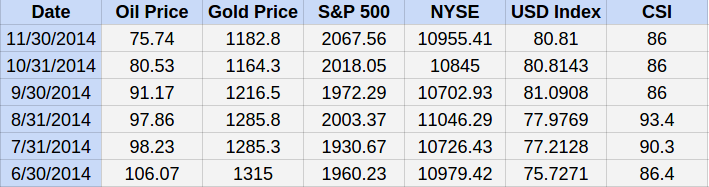
\includegraphics[width=\textwidth]{DataMatrices.png}
\caption{Data frame for oil and gold price and its related macroeconomic factors}
\label{fig:DataMatrices.png}
\end{figure}

\noindent Before calculating the heat map of correlation for oil and gold prices, we have all the prices and macroeconomic factors inflation adjusted.

\begin{figure}
\centering
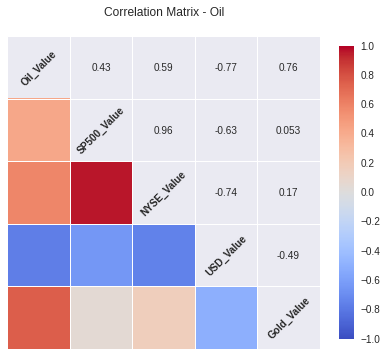
\includegraphics[width=\textwidth]{Correlation_Oil_Value_.png}
\caption{Correlation Heat Map for Oil Price and related macroeconomic factors}
\label{fig:Correlation_Oil_Value_.png}
\end{figure}

\begin{table}
\begin{center}
\begin{tabular}{|c|c|c|c|c|}
\hline
$ $ & $ S\&P\ 500 $ & $ NYSE $ & $ USD\ Index $ & $Gold\ Price$ \\ \hline
$Oil Price$ & $0.43$ & $0.59$ & $-0.77$ & $0.76$ \\ \hline
\end{tabular}
\end{center}
\caption{Correlation Matrix - Oil}
\end{table}

\begin{figure}
\centering
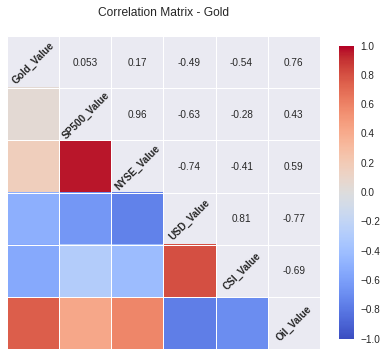
\includegraphics[width=\textwidth]{Correlation_Gold_Value_.png}
\caption{Correlation Heat Map for Oil Price and related macroeconomic factors}
\label{fig:Correlation_Gold_Value_.png}
\end{figure}

\begin{table}
\begin{center}
\begin{tabular}{|c|c|c|c|c|c|}
\hline
$ $ & $ S\&P 500 $ & $ NYSE $ & $ USD $  & $CSI$ &$Oil Price$ \\  \hline
$Gold Price$ & $0.053$ & $0.17$ & $-0.49$ & $-0.54$ & $0.76$ \\ \hline
\end{tabular}
\end{center}
\caption{Correlation Matrix - Gold}
\end{table}

\newpage
\noindent The correlation heat map in \autoref{fig:Correlation_Oil_Value_.png} and \autoref{fig:Correlation_Gold_Value_.png}, and the corresponding tables containing correlation coefficients show the correlation between the price of oil/gold and related economic factors. \\

\noindent This time, we have all the values of the two commodity prices and necessary macroeconomic factors adjusted by inflation. For the oil price, the correlation between the oil price and S\&P 500 is dropped from 0.72 to 0.43, the correlation between the oil price and NYSE index is dropped from 0.81 to 0.59, and the correlation between the oil price and gold price is dropped from 0.87 to 0.76. Similarly, for the gold price, the correlation between the gold price and S\&P 500 is dropped from 0.53 to 0.053, the correlation between the gold price and NYSE index is dropped from 0.59 to 0.17, the absolute value of the correlation between the gold price and the US dollar index is dropped from 0.75 to 0.49, and and the correlation between the gold price and oil price is dropped from 0.87 to 0.76. By doing inflation adjustment, we are certain to have increased the predicing power of our autoregressive with multiple linear regression models. For details, refer to Section 7 Advanced Models. \\

\noindent Our goal is to predict the prices of oil and gold on January 1st, 2015 as of December 1st, 2014, which is a month in advance. Therefore, we have used monthly data, i.e, oil/gold price and values of other economic factors on the last day of every month. But this severely limits the amount of data we can obtain. Although we collected data for the past 30 years, we have just 360 entries in our time series, which isn't a good enough number to generate good enough error metrics. This also limits our prediction power. \\


\section{Observations}

Report on interesting things you can learn/visualize from your data set.  Include and describe these visualizations.  (2-4 pages)


\section{Baseline Models}
In order to illustrate an improvement in the accuracy of our predictions, we compare our advanced models (see Section 7 Advanced Models for details) to the following two baseline models:

\begin {itemize}
\item \textbf{Baseline Model 1} The price is the same as the previous month's price: \\
$P_{t}$ = $P_{t-1}$\\
\item \textbf{Baseline Model 2} The price is a cubic weighted average of the last 3 months: \\
$P_{t}$ = $\frac{1}{\{k(k+1)\}^2}\sum\limits_{i=1}^k (k-i+1)^3P_{t-i}$
\end {itemize}

\subsubsection {Error Metrics of Baseline Models for Oil} 
The following are the error metrics and the error histograms for our baseline models for predicing the oil price:

\begin{table}
\begin{center}
\begin{tabular}{|c|c|c|c|c|c}
\hline
Model & Relative Error & Mean Absolute Error & RMSE & Std Dev of Err \% & Probability \\ \hline
$ Baseline\ Model\ 1 $ & $6.58$ & $5.93$ & $7.85$ & $0.0904$ & $0.7851$ \\ \hline
$ Baseline\ Model\ 2 $ & $7.17$ & $6.37$ & $8.58$ & $0.1025$ & $0.8037$\\ \hline
\end{tabular}
\end{center} 
\caption{Error Metrics for Baseline Model - Oil. 
RMSE stands for Root Mean Squared Error; Probability refers to the probability that the error is within 1 standard deviation}
\end{table}

\begin{figure}
\centering
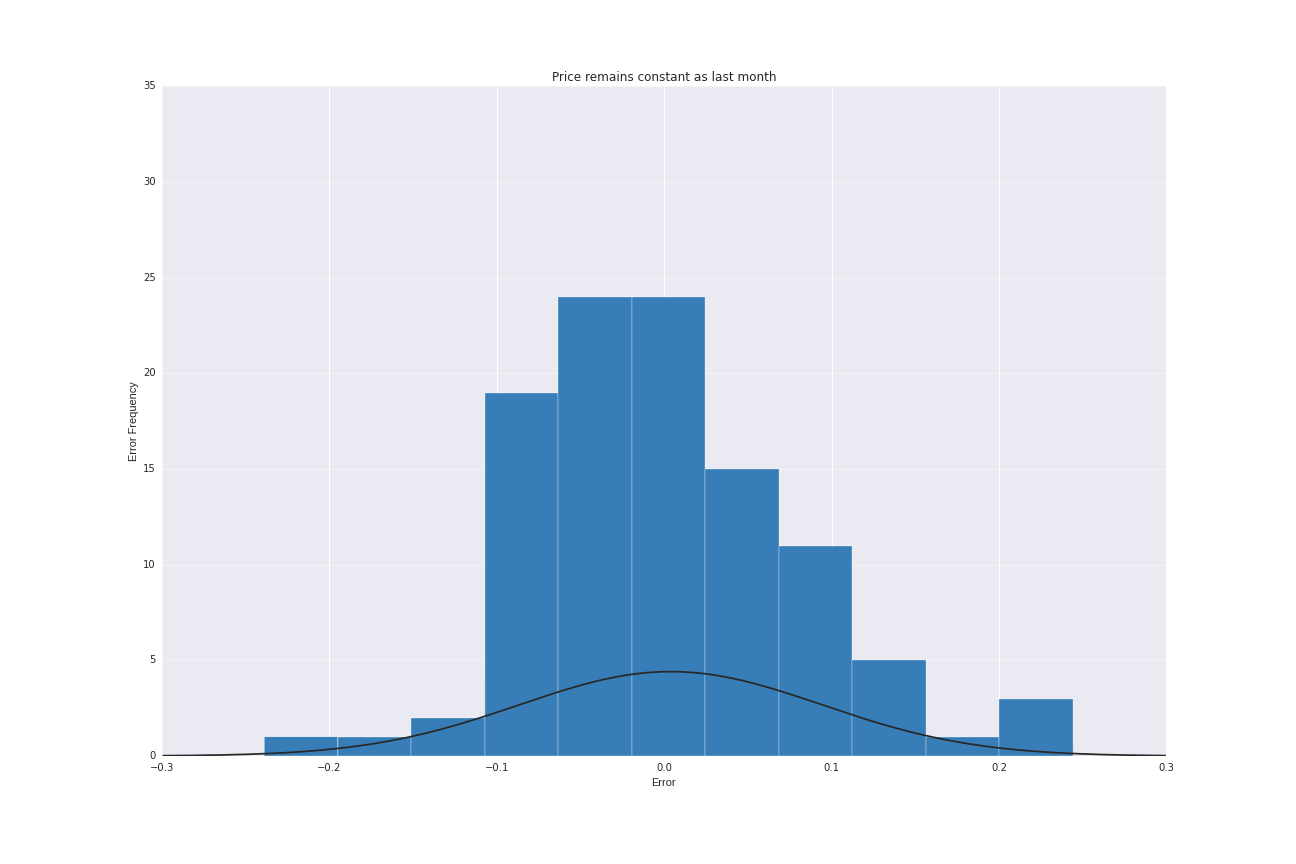
\includegraphics[width=\textwidth]{BM1_Oil.png}
\caption{Error plot for Baseline Model 1 - Oil price is the same as the previous month's price}
\label{fig:BM1_Oil.png}
\end{figure}

\begin{figure}
\centering
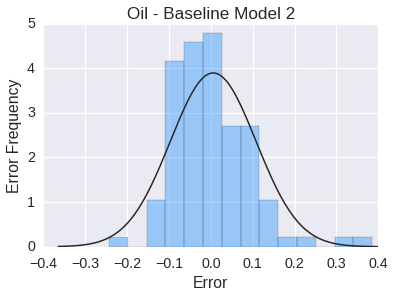
\includegraphics[width=\textwidth]{BM2_Oil.png}
\caption{Error plot for Baseline Model 2 - Oil price is a cubic weighted average of the last 3 months}
\label{fig:BM2_Oil.png}
\end{figure}

\noindent The predicted price of WTI Crude Oil on Jan 1, 2015 as of Dec 1, 2014 is \textbf{75.74 USD per Barrel} based on Baseline Model 1.\\

\noindent The predicted price of WTI Crude Oil on Jan 1, 2015 as of Dec 1, 2014 is \textbf{76.99 USD per Barrel} based on Baseline Model 2.\\

\subsubsection {Error Metrics of Baseline Models for Gold} 
The following are the error metrics and the error histograms for our baseline models for predicing the gold price:

\begin{table}
\begin{center}
\begin{tabular}{|c|c|c|c|c|c}
\hline
Model & Relative Error & Mean Absolute Error & RMSE & Std Dev of Err \% & Probability \\ \hline
$ Baseline\ Model\ 1 $ & $4.61$ & $56.11$ & $75.36$ & $0.0603$ & $0.7196$ \\ \hline
$ Baseline\ Model\ 2 $ & $4.56$ & $55.78$ & $73.27$ & $0.0586$ & $0.6916$\\ \hline
\end{tabular}
\end{center} 
\caption{Error Metrics for Baseline Model - Gold. 
RMSE stands for Root Mean Squared Error; Probability refers to the probability that the error is within 1 standard deviation}
\end{table}

\begin{figure}
\centering
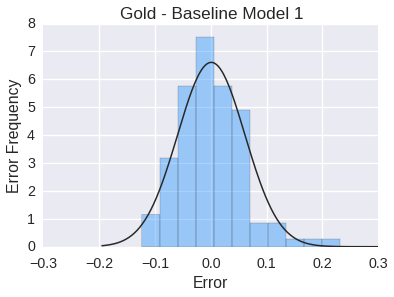
\includegraphics[width=\textwidth]{BM1_Gold.png}
\caption{Error plot for Baseline Model 1 - Gold price is the same as the previous month's price}
\label{fig:BM1_Gold.png}
\end{figure}

\begin{figure}
\centering
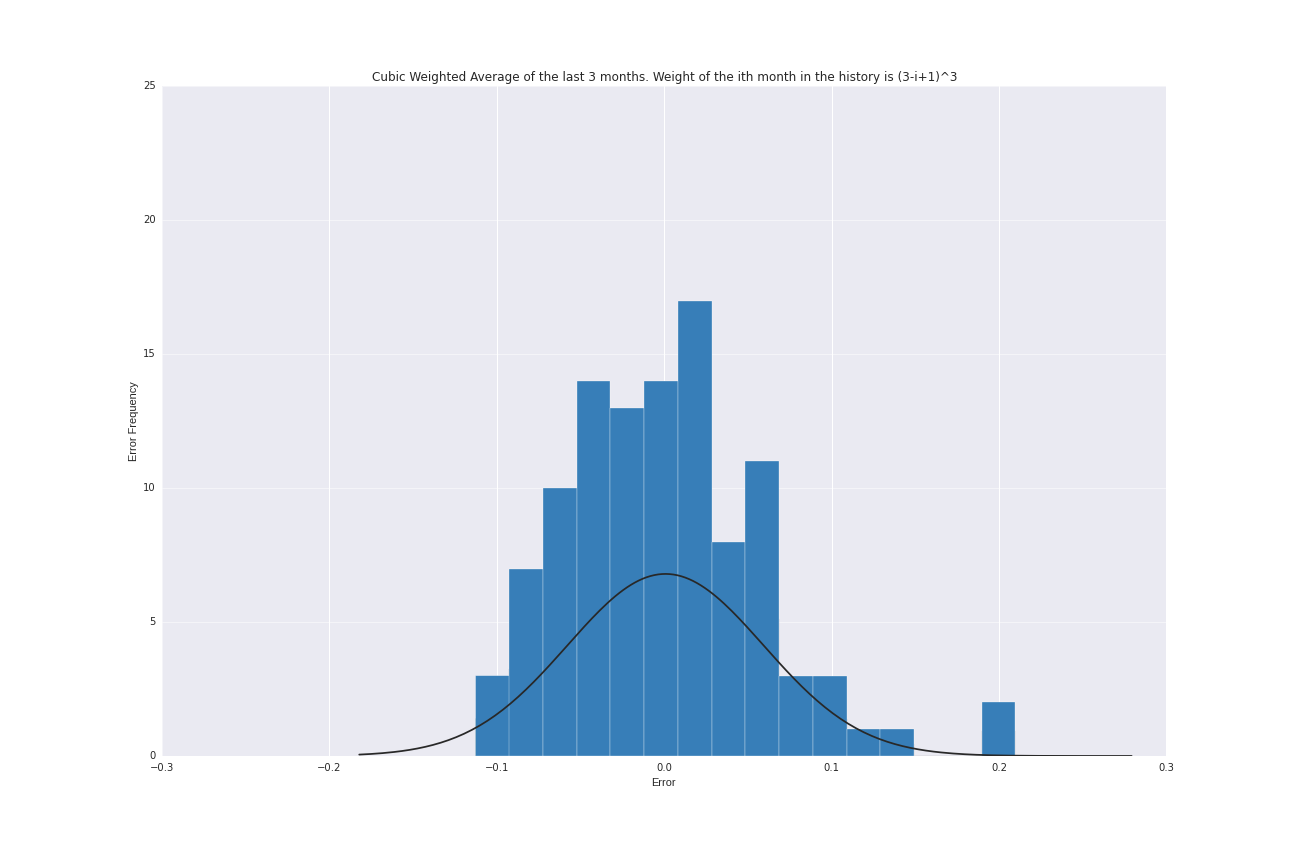
\includegraphics[width=\textwidth]{BM2_Gold.png}
\caption{Error plot for Baseline Model 2 - Gold price is a cubic weighted average of the last 3 months}
\label{fig:BM2_Gold.png}
\end{figure}

\noindent The predicted price of Gold Jan 1, 2015 as of Dec 1, 2014 is 
\textbf{1182.80 USD per ounce} based on Baseline Model 1.\\

\noindent The predicted price of Gold Jan 1, 2015 as of Dec 1, 2014 is 
\textbf{1179.84 USD per ounce} based on Baseline Model 2.\\

\section{Advanced Models}
We have developed autoregressive, autoregressive with multiple linear regression, and regression using futures data models to make our predictions on oil and gold prices. \\

\subsection{Autoregressive Models}
\noindent\textbf{Standard Autoregressive Model} This model is purely based on the historical prices. It models the time series as a linear function of the values of the past 'p' months.\\

$ X_{t} = c + \sum\limits_{i=1}^p \varphi_{t-i}X_{t-i}$. \\

\noindent The Ordinary Least Squares (OLS) method is used to estimate the parameters of the regression function. It tries to minimize the sum of squares of vertical distances between the predicted and the actual values. \\

\noindent\textbf{ARMA} ARMA models are used to understand and predict time series values as a function of two polynomials, an autoregressive function, and a moving average function. 
\\

$ X_{t} = c + \sum\limits_{i=1}^p \varphi_{t-i}X_{t-i} + \epsilon_{t} + \sum\limits_{i=1}^q \theta_{t-i}X_{t-i}$.\\

\noindent In ARMA (p,q), p is referred to as the order of the autoregressive part and q is referred to as the order of the moving average part, i.e, the model is described using p autoregressive terms and q moving average terms.\\ 

\subsection{Autoregressive with Multiple Linear Regression Models}
Linear regression models the relationship between two variables - a dependent variable and an explanatory variable using a linear function. The process of modelling a variable based on more than one explanatory variables is called Multiple Linear Regression. \\
   
\noindent We initially develop a model which generates a purely autoregressive function. Then, the model is expanded to incorporate the factors which are highly correlated to the price of oil/gold we are trying to predict. As each factor is incorporated into the model, we perform a comparison of the error metrics between these models and try to estimate the model which makes predictions with a better accuracy.\\

\noindent For predicting the price of oil, the following macroeconomic factors are taken into consideration:
\begin {itemize}
\item S\&P 500 Index
\item NYSE Index
\item US Dollar Index
\item Gold Price
\end {itemize}

\noindent For predicting the price of gold, the following factors macroeconomic are taken into consideration:
\begin {itemize}
\item S\&P 500 Index
\item NYSE Index
\item US Dollar Index
\item Consumer Sentiment Index
\item Oil Price
\end {itemize}

\subsection{Regression using Futures Data Models}
TODO

\subsection{Oil Price Prediction}
The following graph shows the comparison of the relative errors of our Autoregressive Models and Autoregressive with Multiple Linear Regression Models for the oil price prediction.

\begin{figure}
\centering
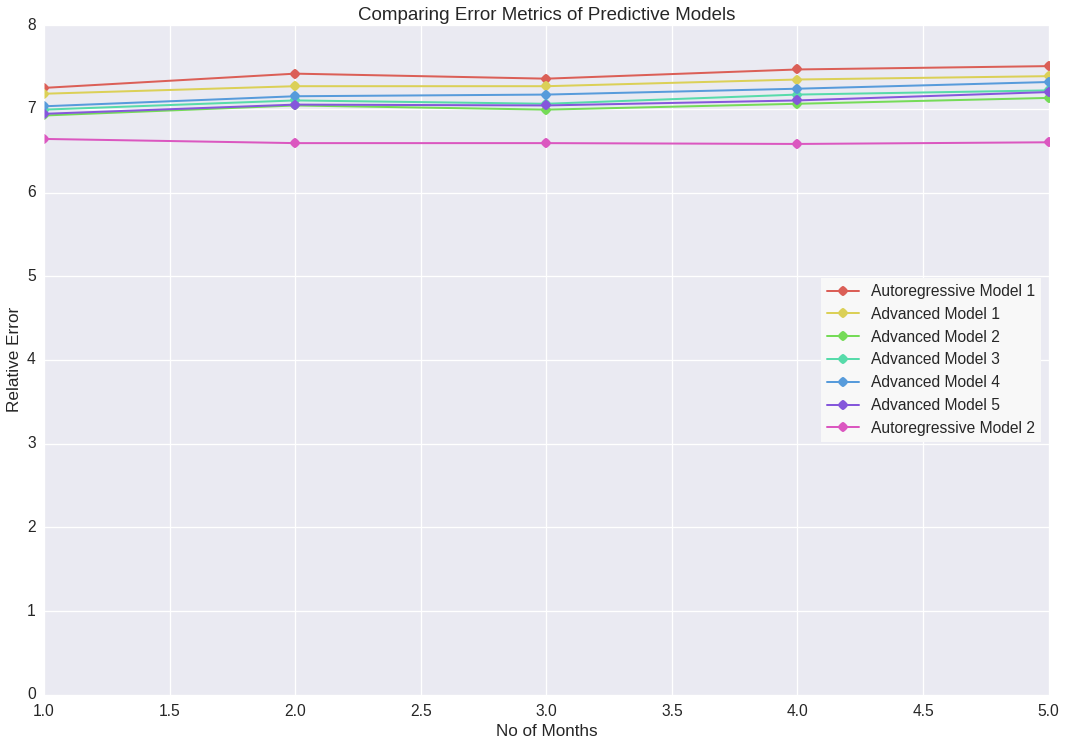
\includegraphics[width=\textwidth]{ModelComparison_Oil.png}
\caption{Performance of the standard autoregressive model, ARMA model and the autoregressve with multiple linear regression models}
\label{fig:ModelComparison_Oil.png}
\end{figure}

\begin{figure}
\centering
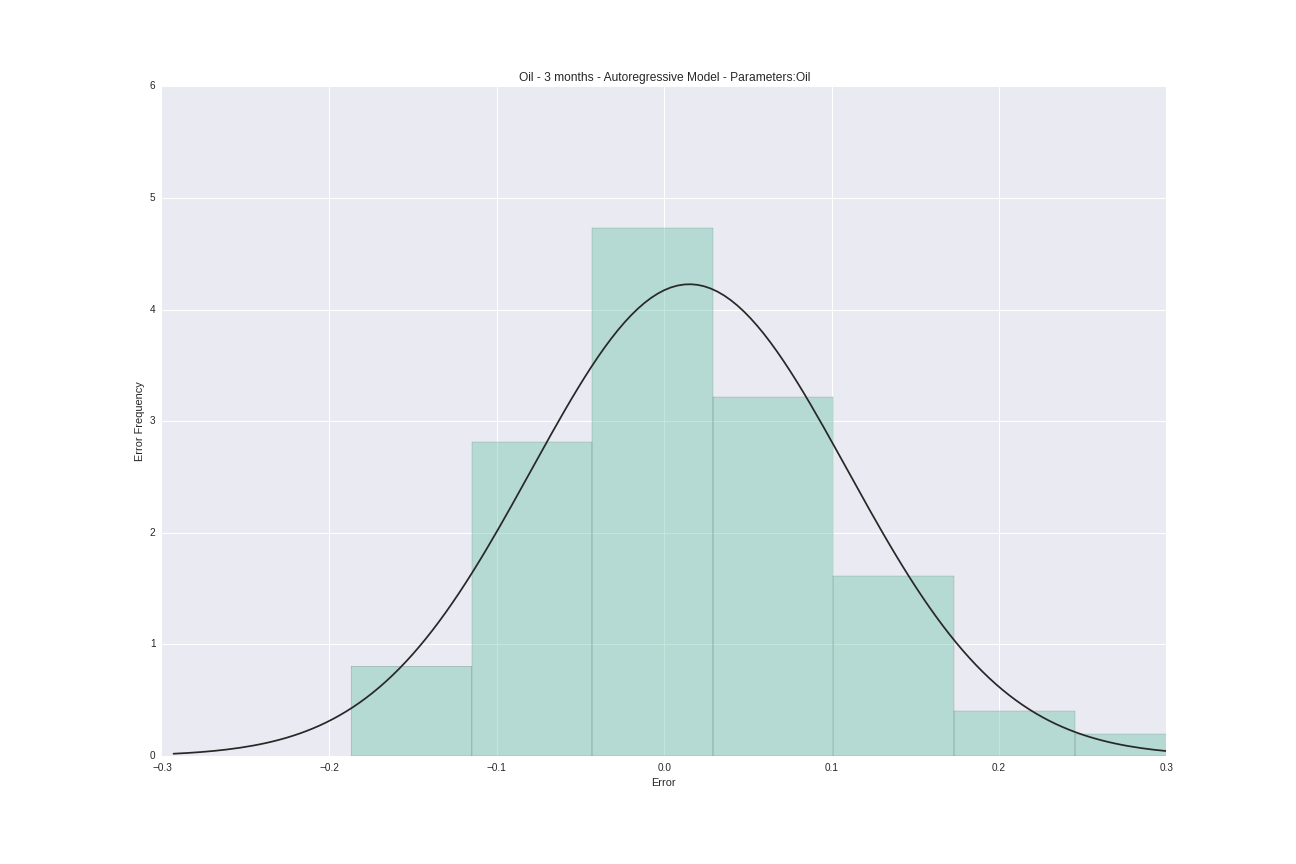
\includegraphics[width=\textwidth]{Oil_Auto.png}
\caption{Oil: The Relative Error Distribution for the Standard Autoregressive Model}
\label{fig:Oil_Auto.png}
\end{figure}

\begin{figure}
\centering
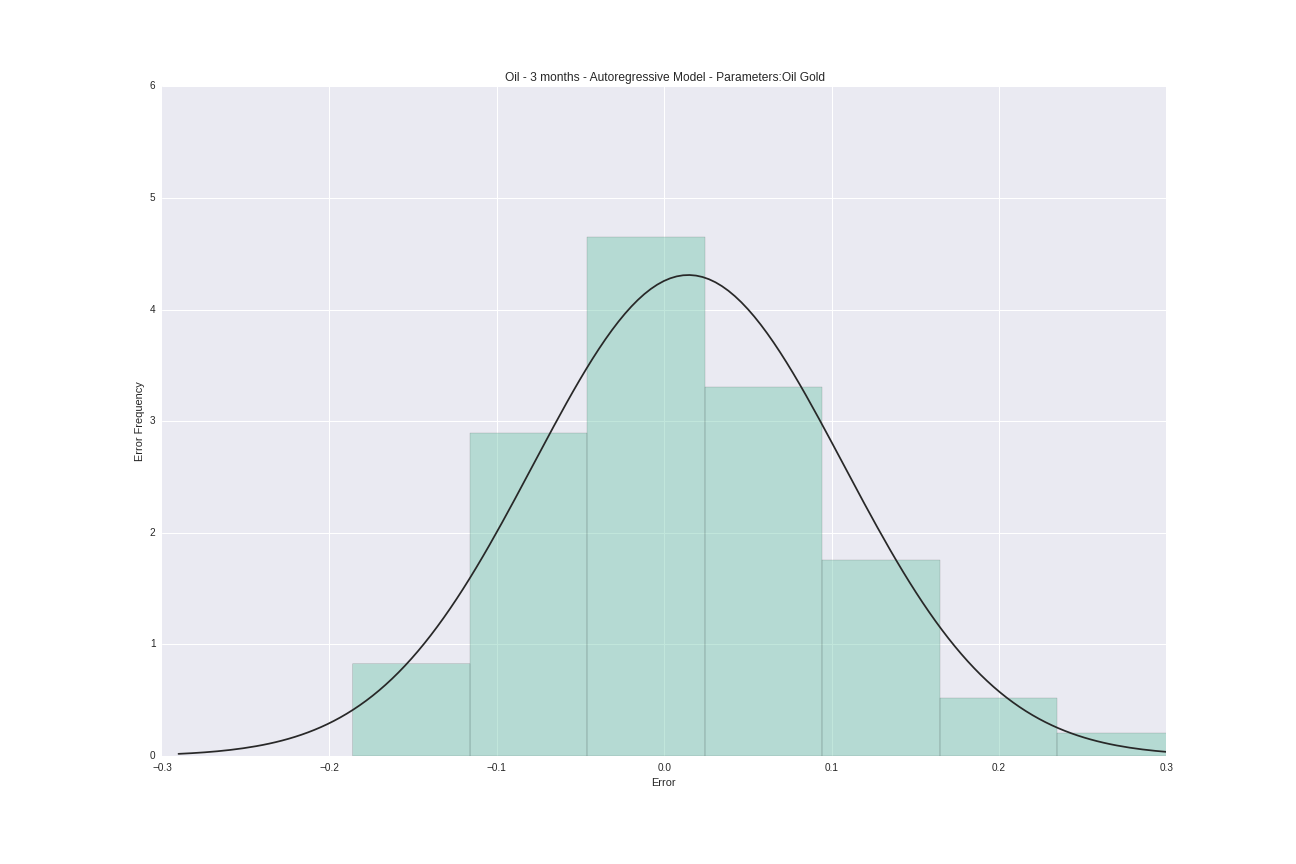
\includegraphics[width=\textwidth]{Oil_Gold.png}
\caption{Oil: The Autoregressive with Multiple Linear Regression Model with One Economic Factor - Gold}
\label{fig:Oil_Gold.png}
\end{figure}

\begin{figure}
\centering
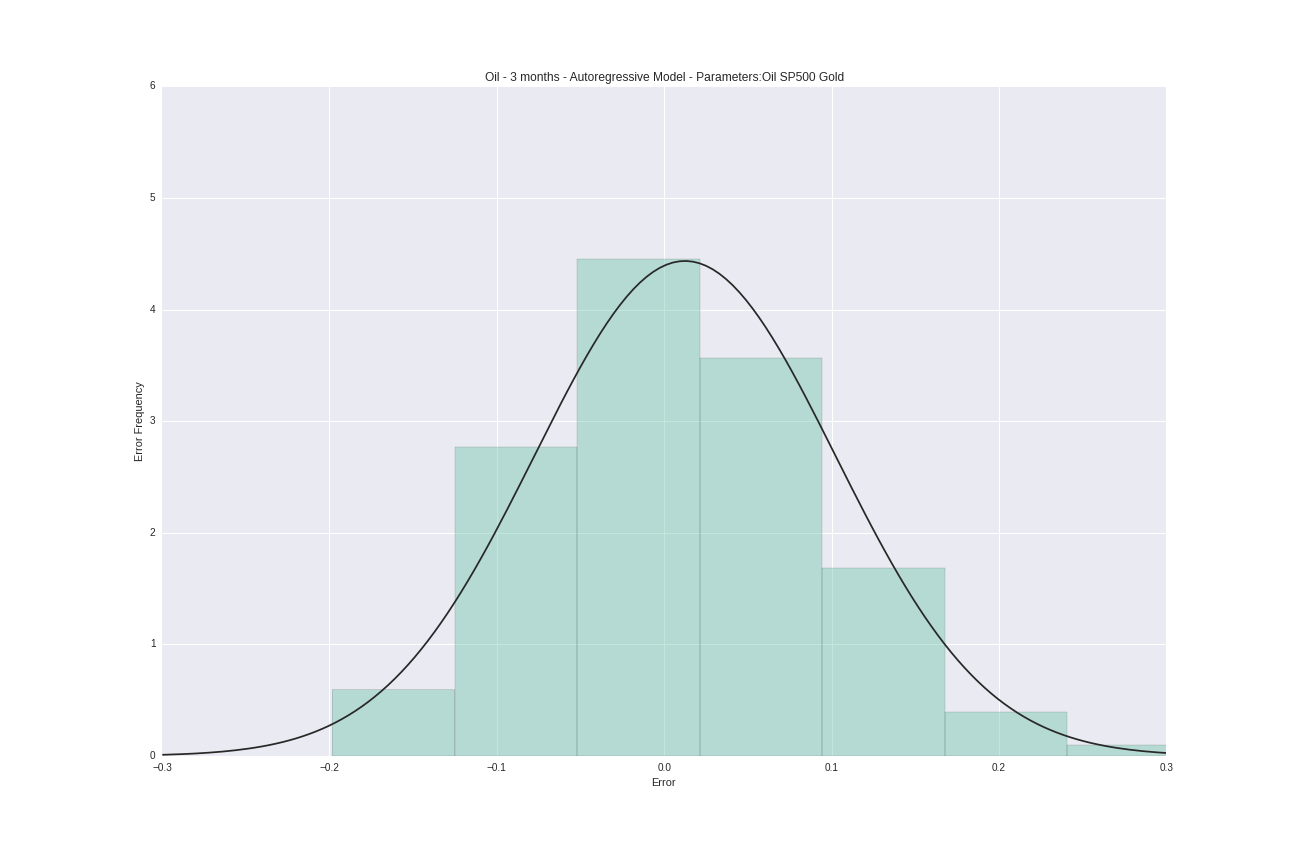
\includegraphics[width=\textwidth]{Oil_SP500_Gold.png}
\caption{Oil: The Autoregressive with Multiple Linear Regression Model with Two Economic Factors - SP500 and Gold}
\label{fig:Oil_SP500_Gold.png}
\end{figure}

\begin{figure}
\centering
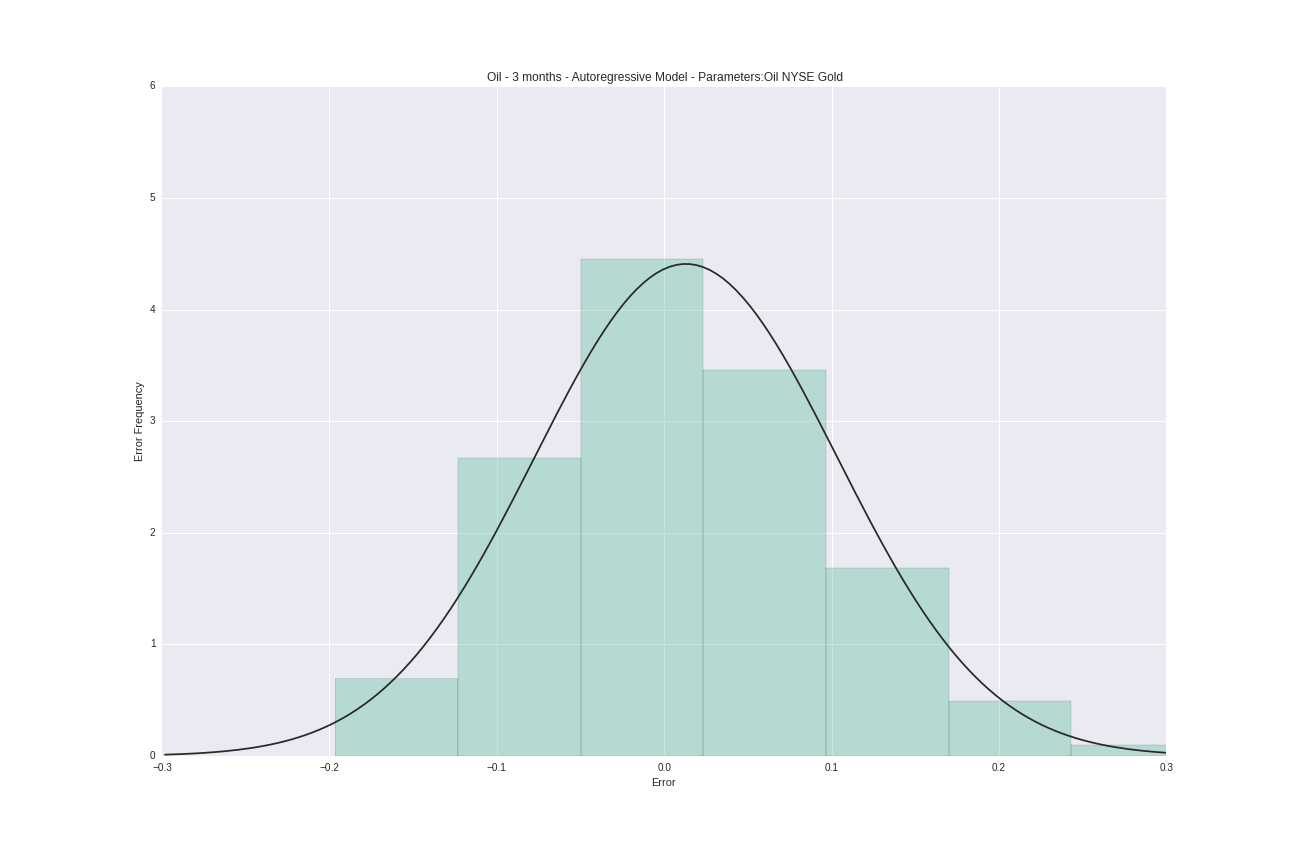
\includegraphics[width=\textwidth]{Oil_NYSE_Gold.png}
\caption{Oil: The Autoregressive with Multiple Linear Regression Model with Two Economic Factors - NYSE and Gold}
\label{fig:Oil_NYSE_Gold.png}
\end{figure}

\begin{figure}
\centering
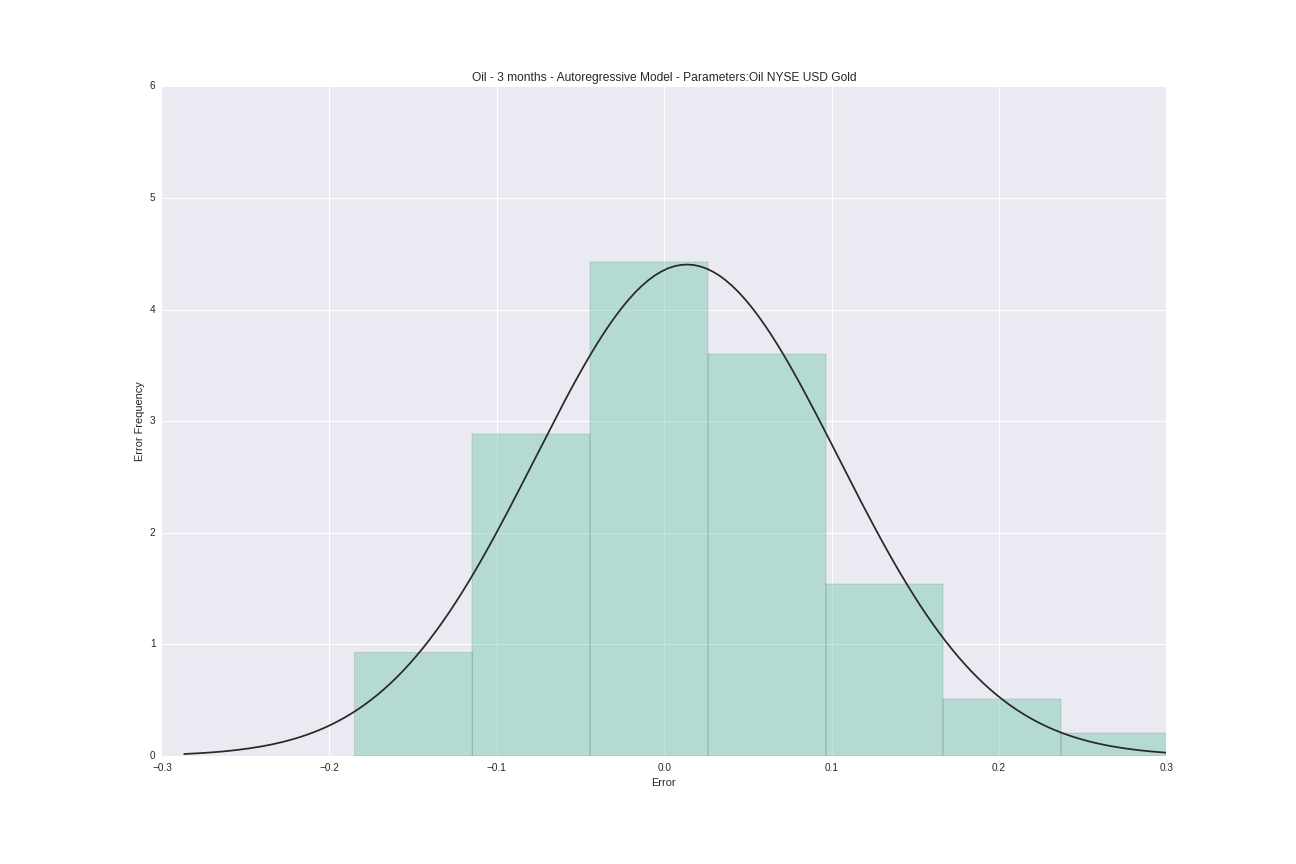
\includegraphics[width=\textwidth]{Oil_NYSE_USD_Gold.png}
\caption{Oil: The Autoregressive with Multiple Linear Regression Model with Three Economic Factors - NYSE, USD and Gold}
\label{fig:Oil_NYSE_USD_Gold.png}
\end{figure}

\begin{figure}
\centering
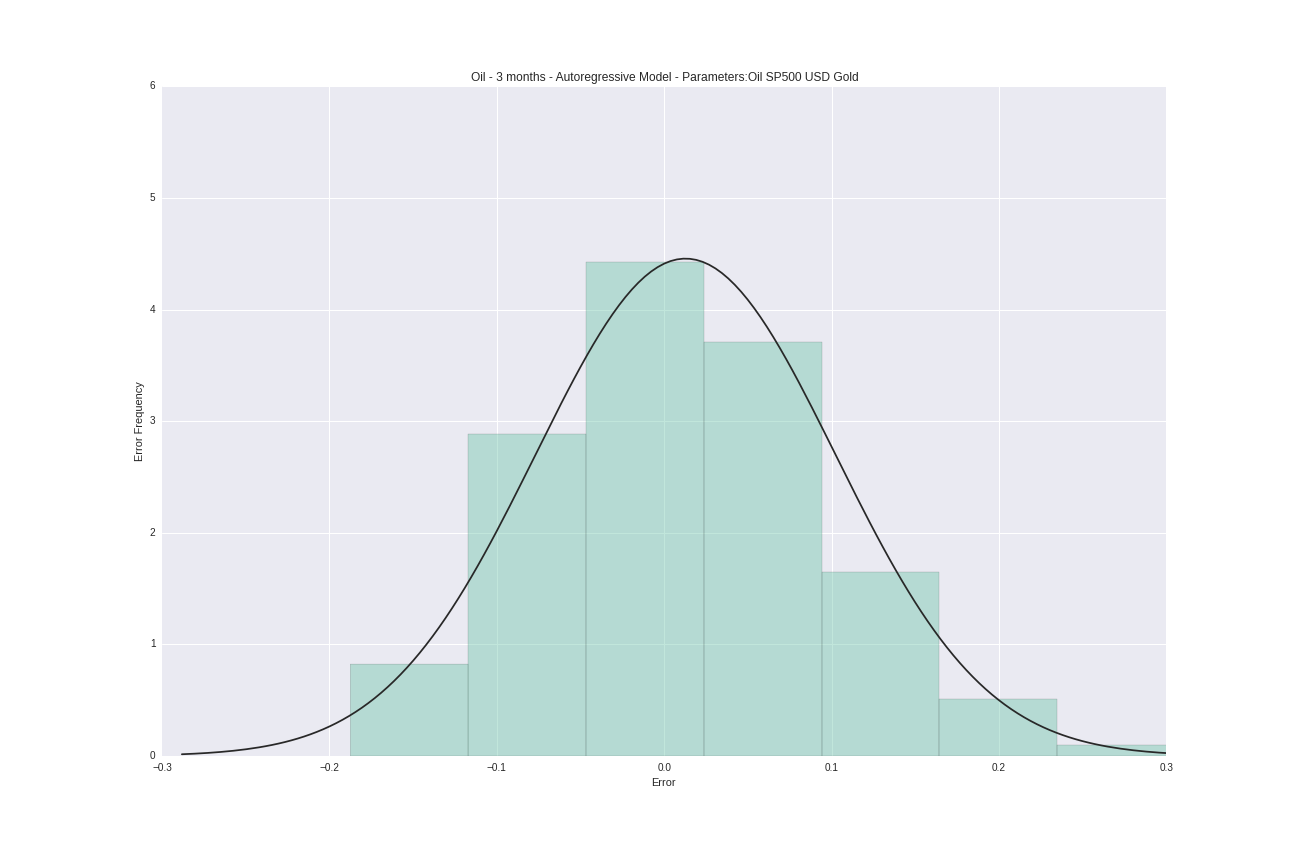
\includegraphics[width=\textwidth]{Oil_SP500_USD_Gold.png}
\caption{Oil: The Autoregressive with Multiple Linear Regression Model with Three Economic Factors - SP500, USD and Gold}
\label{fig:Oil_SP500_USD_Gold.png}
\end{figure}

\noindent Below is a summary of all the models we used for predicting the oil price (For convenience, we include the two baseline models in Secion 6 as well) \\

\begin{table}
\begin{center}
\begin{tabular}{|c|c|c|c|c|c}
\hline
Model & Relative Error & Mean Absolute Error & RMSE & Std Dev of Err \% & Probability \\ \hline
$ Baseline\ Model\ 1 $ & $6.58$ & $5.93$ & $7.85$ & $0.0904$ & $0.7851$ \\ \hline
$ Baseline\ Model\ 2 $ & $7.17$ & $6.37$ & $8.58$ & $0.1025$ & $0.8037$\\ \hline
$ Standard\ Autoregressive $ & $7.36$ & $5.73$ & $7.29$ & $0.0944$ & $0.7174$\\ \hline
$ ARMA $ & $6.78$ & $5.03$ & $5.42$ & $0.0846$ & $0.7410$\\ \hline
$ MLR:\ Gold $ & $7.27$ & $5.67$ & $7.21$ & $0.0926$ & $0.7101$\\ \hline
$ MLR:\ SP500,\ Gold $ & $6.99$ & $5.52$ & $7.16$ & $0.0899$ & $0.7174$\\ \hline
$ MLR:\ NYSE,\ Gold $ & $7.06$ & $5.56$ & $7.16$ & $0.0905$ & $0.7101$\\ \hline
$ MLR:\ NYSE,\ USD,\ Gold $ & $7.17$ & $5.61$ & $7.14$ & $0.0906$ & $0.7029$\\ \hline
$ MLR:\ SP500,\ USD,\ Gold $ & $7.04$ & $5.54$ & $7.12$ & $0.0895$ & $0.7101$\\ \hline
$ Using\ Futures $ & $3.75$ & $3.08$ & $4.34$ & $0.0515$ & TBC \\ \hline
\end{tabular}
\end{center} 
\caption{Error Metrics of various models for predicting the oil price.
RMSE stands for Root Mean Squared Error; Probability refers to the probability that the error is within 1 standard deviation; MLR stands for Multiple Linear Regression, the name(s) after MLR is the macroeconomic factor(s) used in the model}
\end{table} 

\noindent\textbf{Summary}

\subsection{Gold Price Prediction}
The following graph shows the comparison of the relative errors of our Autoregressive Models and Autoregressive with Multiple Linear Regression Models for the gold price prediction.

\begin{figure}
\centering
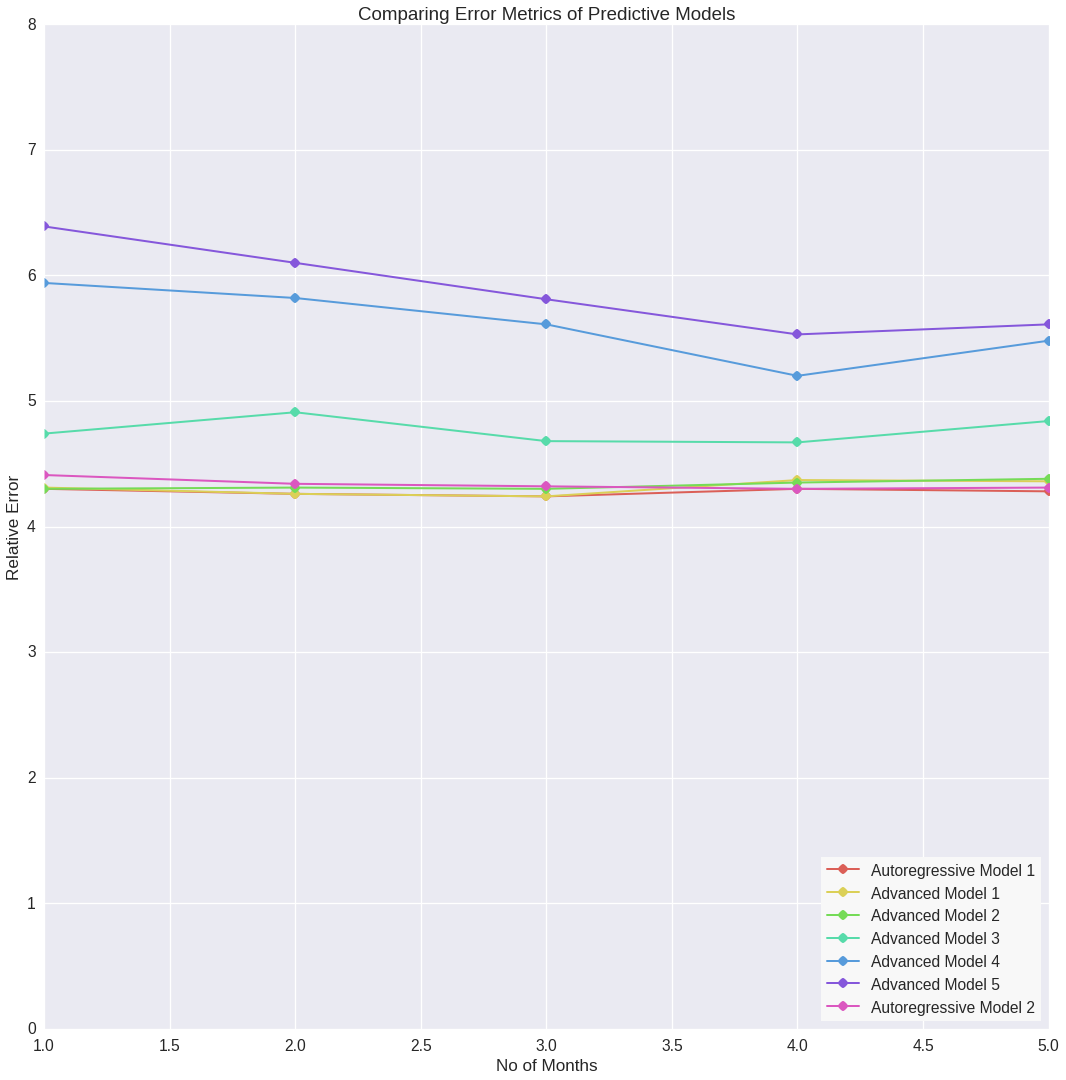
\includegraphics[width=\textwidth]{ModelComparison_Gold.png}
\caption{Performance of the standard autoregressive model, ARMA model and the autoregressve with multiple linear regression models}
\label{fig:ModelComparison_Gold.png}
\end{figure}

\begin{figure}
\centering
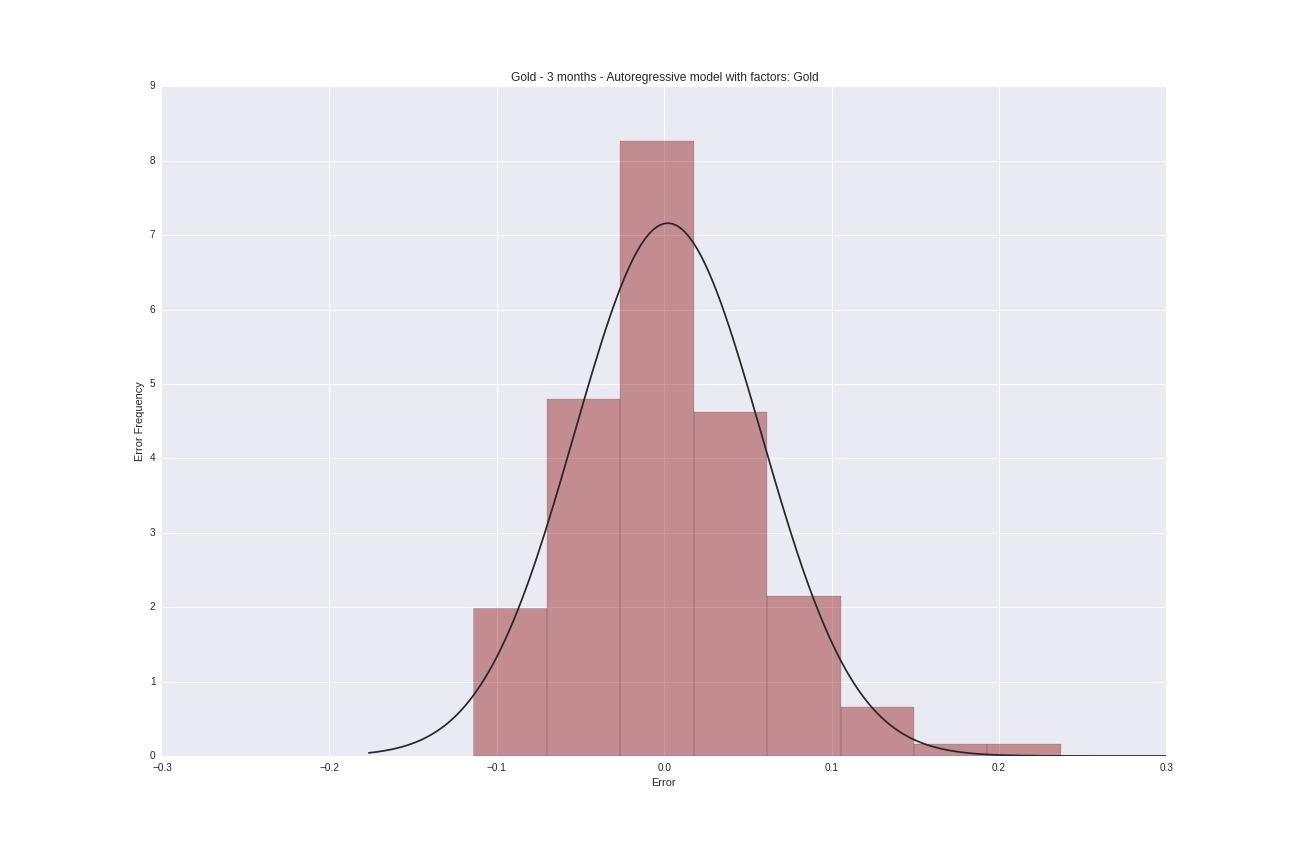
\includegraphics[width=\textwidth]{Gold_Auto.png}
\caption{Gold: The Relative Error Distribution for the Standard Autoregressive Model}
\label{fig:Gold_Auto.png}
\end{figure}

\begin{figure}
\centering
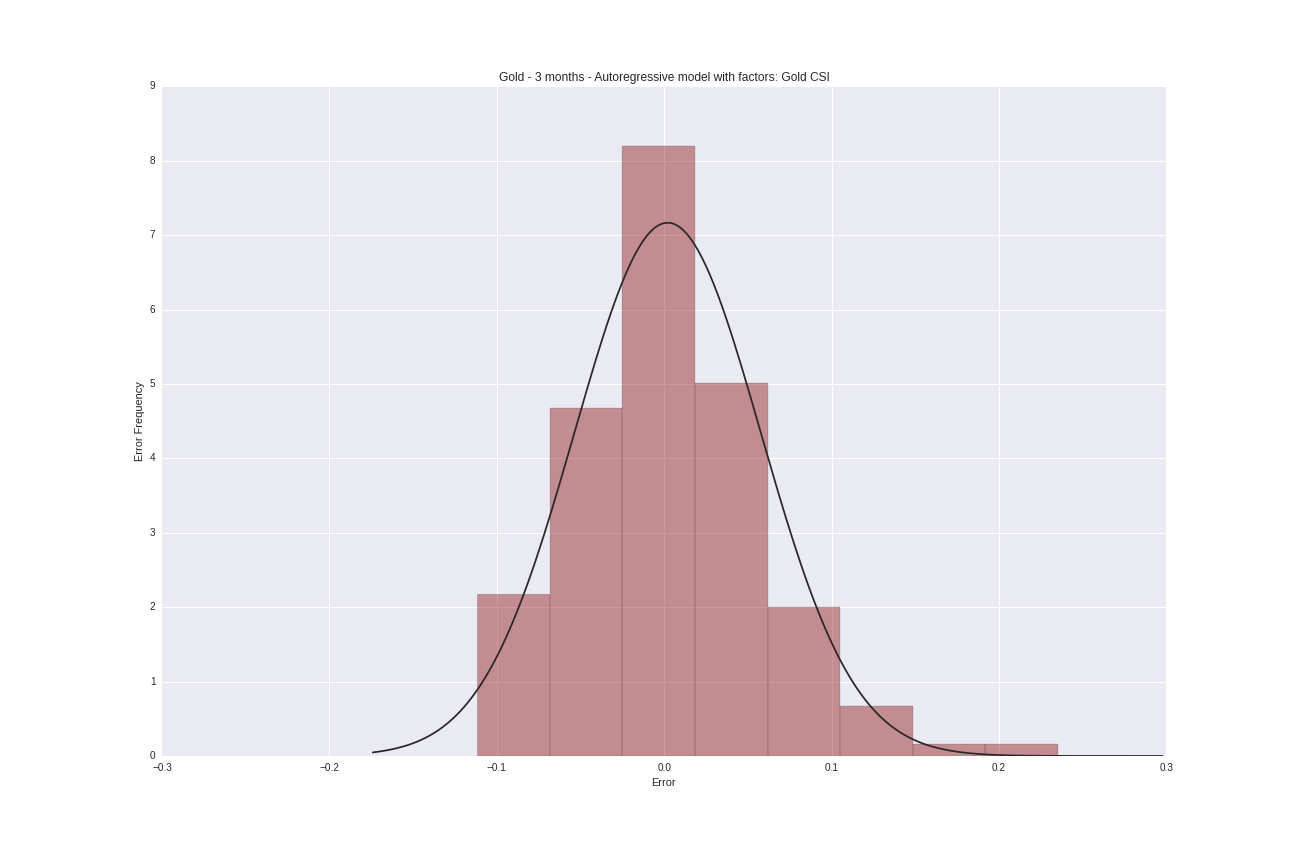
\includegraphics[width=\textwidth]{Gold_CSI.png}
\caption{Gold: The Autoregressive with Multiple Linear Regression Model with One Economic Factor - CSI}
\label{fig:Gold_CSI.png}
\end{figure}

\begin{figure}
\centering
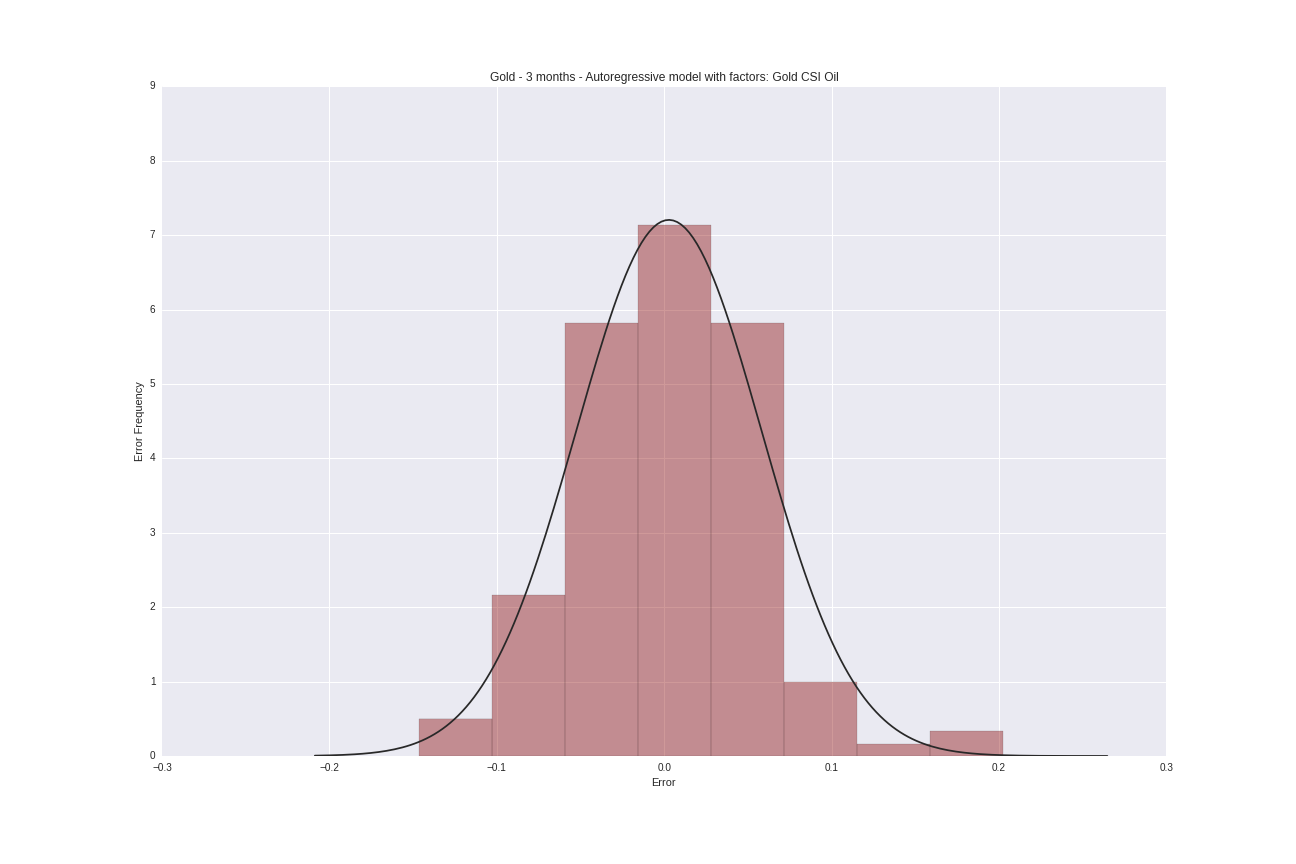
\includegraphics[width=\textwidth]{Gold_CSI_Oil.png}
\caption{Gold: The Autoregressive with Multiple Linear Regression Model with Two Economic Factors - CSI and Oil}
\label{fig:Gold_CSI_Oil.png}
\end{figure}

\begin{figure}
\centering
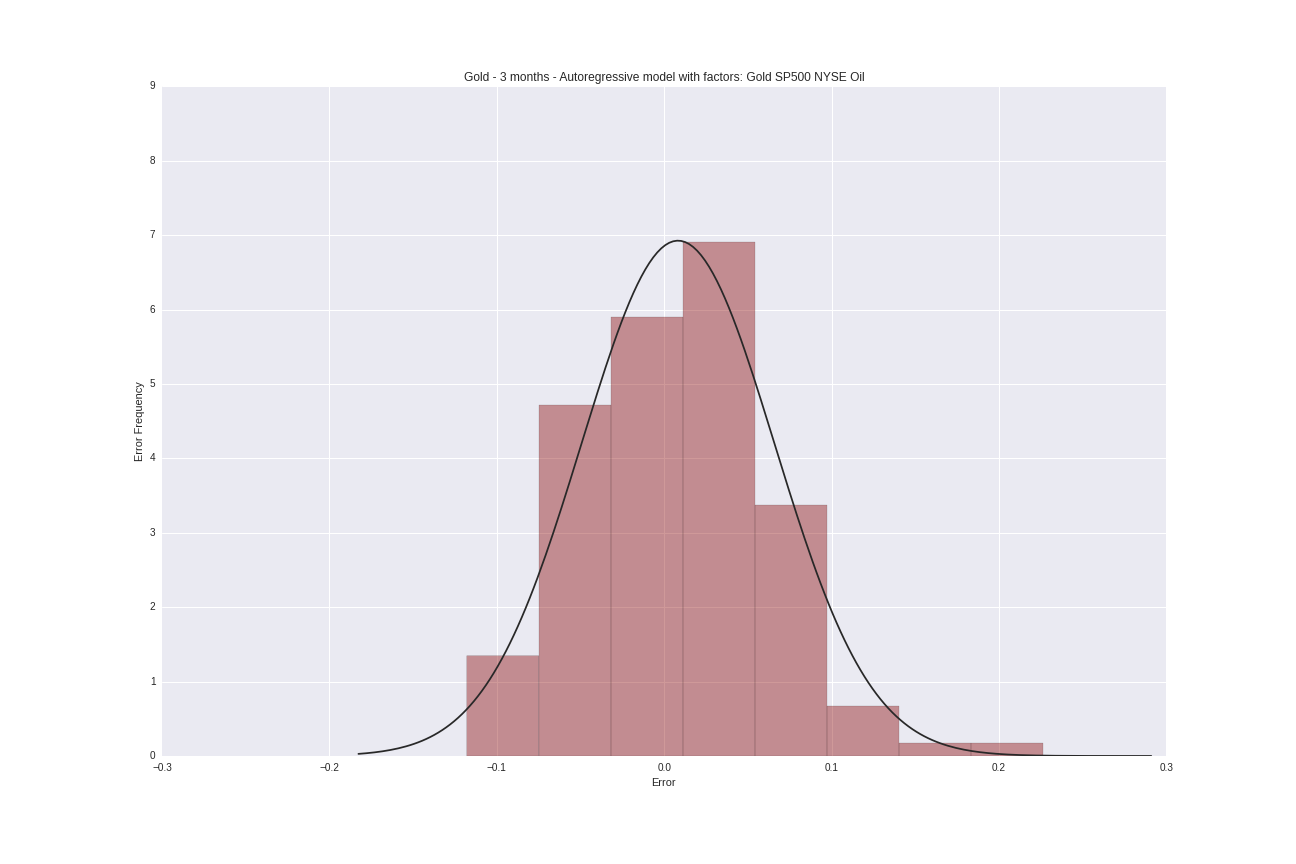
\includegraphics[width=\textwidth]{Gold_SP500_NYSE_Oil.png}
\caption{Gold: The Autoregressive with Multiple Linear Regression Model with Three Economic Factors - SP500, NYSE and Oil}
\label{fig:Gold_SP500_NYSE_Oil.png}
\end{figure}

\begin{figure}
\centering
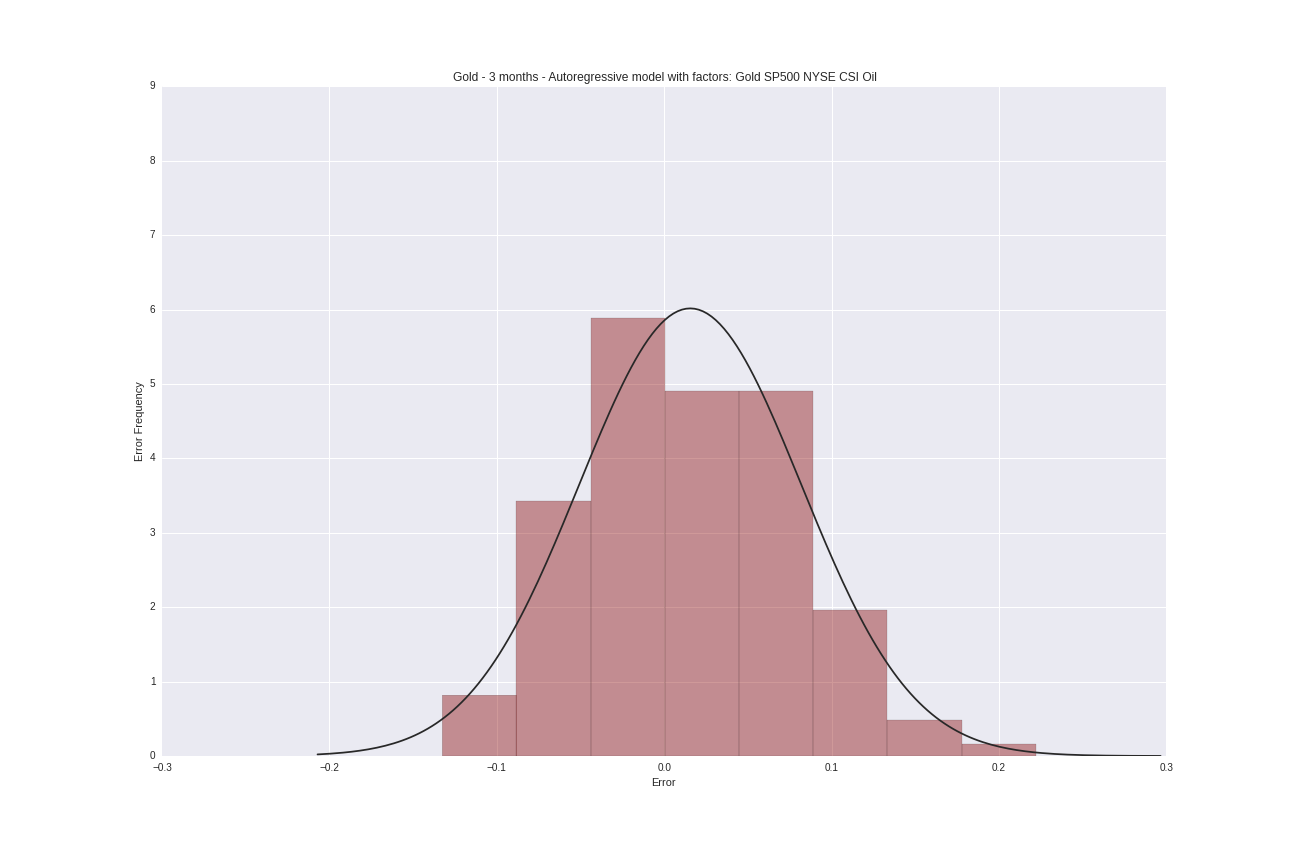
\includegraphics[width=\textwidth]{Gold_SP500_NYSE_CSI_Oil.png}
\caption{Gold: The Autoregressive with Multiple Linear Regression Model with Four Economic Factors - SP500, NYSE, CSI and Oil}
\label{fig:Gold_SP500_NYSE_CSI_Oil.png}
\end{figure}

\begin{figure}
\centering
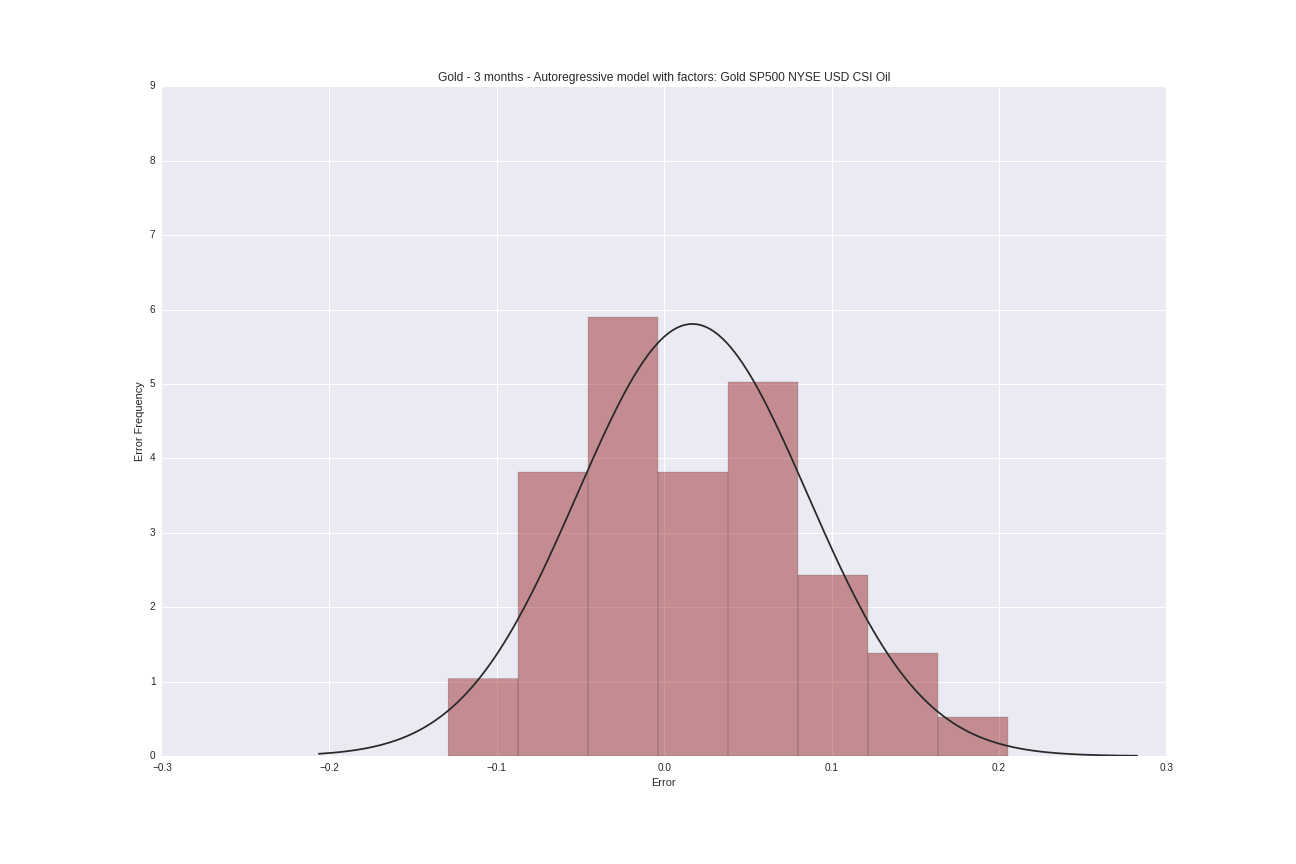
\includegraphics[width=\textwidth]{Gold_SP500_NYSE_USD_CSI_Oil.png}
\caption{Gold: The Autoregressive with Multiple Linear Regression Model with Five Economic Factors - SP500, NYSE, USD, CSI and Oil}
\label{fig:Gold_SP500_NYSE_USD_CSI_Oil.png}
\end{figure}

\noindent Below is a summary of all the models we used for predicting the oil price (For convenience, we include the two baseline models in Secion 6 as well) \\

\begin{table}
\begin{center}
\begin{tabular}{|c|c|c|c|c|c}
\hline
Model & Relative Error & Mean Absolute Error & RMSE & Std Dev of Err \% & Probability \\ \hline
$ Baseline\ Model\ 1 $ & $4.61$ & $56.11$ & $75.36$ & $0.0603$ & $0.7196$ \\ \hline
$ Baseline\ Model\ 2 $ & $4.56$ & $55.78$ & $73.27$ & $0.0586$ & $0.6916$\\ \hline
$ Standard\ Autoregressive $ & $4.24$ & $46.61$ & $65.91$ & $0.0557$ & $0.7029$\\ \hline
$ ARMA $ & $4.32$ & $45.73$ & $63.71$ & $0.0554$ & $0.6966$\\ \hline
$ MLR:\ CSI $ & $4.24$ & $46.62$ & $65.87$ & $0.0557$ & $0.7029$\\ \hline
$ MLR:\ CSI,\ Oil $ & $4.3$ & $47.24$ & $65.86$ & $0.0554$ & $0.7029$\\ \hline
$ MLR:\ SP500,\ NYSE,\ Oil $ & $4.68$ & $49.17$ & $65.67$ & $0.0576$ & $0.7029$\\ \hline
$ MLR:\ SP500,\ NYSE,\ CSI,\ Oil $ & $5.61$ & $55.02$ & $69.51$ & $0.0663$ & $0.6667$\\ \hline
$ MLR:\ SP500,\ NYSE,\ USD,\ CSI,\ Oil $ & $5.81$ & $56.09$ & $70.06$ & $0.0687$ & $0.6739$\\ \hline
$ Using\ Futures $ & TBC & TBC & TBC & TBC & TBC \\ \hline
\end{tabular}
\end{center} 
\caption{Error Metrics of various models for predicting the gold price.
RMSE stands for Root Mean Squared Error; Probability refers to the probability that the error is within 1 standard deviation; MLR stands for Multiple Linear Regression, the name(s) after MLR is the macroeconomic factor(s) used in the model}
\end{table} 

\noindent\textbf{Summary}


\section{Final Prediction and Conclusions}
\subsection {Final Prediction}
\noindent The predicted price of WTI Crude Oil on Jan 1, 2015 as of Dec 1, 2014 is \\
\textbf{71.22 USD per Barrel} \\

\noindent The predicted price of Gold on Jan 1, 2015 as of Dec 1, 2014 is \\
\textbf{1179.25 USD per ounce} \\

\subsection {Difficulties We Had to Overcome in Building Good Models}

\begin{itemize}
\item \textbf{Item 1} Item 1
\item \textbf{Item 2} Item 2
\item \textbf{Item 3} Item 3
\end{itemize}

\subsection {Investigations for Subsequent Groups}

\begin{itemize}
\item \textbf{Item 1} Item 1
\item \textbf{Item 2} Item 2
\item \textbf{Item 3} Item 3
\end{itemize}


\subsubsection*{Acknowledgments.} Dr. Steven Skiena. Professor Keli (Andrew) Xiao.

\section{Bibliography}\label{references}

\begin{thebibliography}{4}
\bibitem{opec} "OPEC : Home.". \url{http://www.opec.org/}

\bibitem{eiafactors} "Energy and Financial Markets: What Drives Crude Oil Prices". \url{http://www.eia.gov/finance/markets}

\bibitem{oildollar} Zhang, Yue-Jun, et al. "Spillover effect of US dollar exchange rate on oil prices." Journal of Policy Modeling 30.6 (2008): 973-991.

\bibitem{gold-shafiee} Shahriar Shafiee,  Erkan Topal.:An overview of global gold market and gold price forecasting. ScienceDirect. Volume 35, Issue 3, September 2010, 178--189 (2010)

\bibitem{gold-zhang} Zhang, Yue-Jun, and Yi-Ming Wei. "The crude oil market and the gold market: Evidence for cointegration, causality and price discovery." Resources Policy 35.3 (2010): 168-177.

\bibitem{oil-zhang}Zhang, Xun, Kin Keung Lai, and Shou-Yang Wang. "A new approach for crude oil price analysis based on empirical mode decomposition." Energy Economics 30.3 (2008): 905-918.

\bibitem{gold-Ismail}Z. Ismail, A. Yahya and A. Shabri. "Forecasting Gold Prices Using Multiple Linear Regression Method." American Journal of Applied Sciences 6 (8) (2009): 1509-1514.

\bibitem{gold-url1} The Relationship between Gold and Crude Oil Price, \url{http://www.marketoracle.co.uk/Article38141.html}

\bibitem{csi-1} What's the difference between consumer confidence and consumer sentiment?, \url{http://www.investopedia.com/ask/answers/09/consumer-confidence-sentiment-difference.asp}

\bibitem{csi-1} What's the difference between consumer confidence and consumer sentiment?, \url{http://www.investopedia.com/ask/answers/09/consumer-confidence-sentiment-difference.asp}

\bibitem{csi-2} Consumer confidence index, \url{http://en.wikipedia.org/wiki/Consumer_confidence_index}

\bibitem{engle} Engle, Robert. "GARCH 101: The use of ARCH/GARCH models in applied econometrics." Journal of economic perspectives (2001): 157-168.

\bibitem{gold-pso}Hadavandi, Esmaeil, Arash Ghanbari, and Salman Abbasian-Naghneh. "Developing a Time Series Model Based on Particle Swarm Optimization for Gold Price Forecasting." Business Intelligence and Financial Engineering (BIFE), 2010 Third International Conference on. IEEE, 2010.

\bibitem{gold-ref1}Khashei, Mehdi, Mehdi Bijari, and Gholam Ali Raissi Ardali. "Improvement of auto-regressive integrated moving average models using fuzzy logic and artificial neural networks (ANNs)." Neurocomputing 72.4 (2009): 956-967.

\bibitem{gold-ref2}Khashei, Mehdi, Seyed Reza Hejazi, and Mehdi Bijari. "A new hybrid artificial neural networks and fuzzy regression model for time series forecasting." Fuzzy Sets and Systems 159.7 (2008): 769-786.

\bibitem{huntington} Huntington, Hillard G. "Oil price forecasting in the 1980s: what went wrong?." The Energy Journal (1994): 1-22.

\bibitem{pindyck} Pindyck, Robert S. "The long-run evolution of energy prices." The Energy Journal (1999): 1-27.

\bibitem{dongbing}Dong, Bing, Cheng Cao, and Siew Eang Lee. "Applying support vector machines to predict building energy consumption in tropical region." Energy and Buildings 37.5 (2005): 545-553.

\bibitem{yang} Yang, C. W., Ming-Jeng Hwang, and Bwo-Nung Huang. "An analysis of factors affecting price volatility of the US oil market." Energy Economics 24.2 (2002): 107-119.

\bibitem{quandal} Quandl - Find, Use and Share Numerical Data. \url{https://www.quandl.com}

\bibitem{csi}\url{http://future.aae.wisc.edu/data/monthly_values/by_area/998?grid=true}

\end{thebibliography}

\end{document}
